% Options for packages loaded elsewhere
\PassOptionsToPackage{unicode}{hyperref}
\PassOptionsToPackage{hyphens}{url}
\documentclass[]{article}
\usepackage{xcolor}
\usepackage{amsmath,amssymb}
\setcounter{secnumdepth}{-\maxdimen} % remove section numbering
\usepackage{iftex}
\ifPDFTeX
  \usepackage[T5]{fontenc}
\usepackage[vietnamese]{babel}
  \usepackage[utf8]{inputenc}
  \usepackage{textcomp} % provide euro and other symbols
\else % if luatex or xetex
  \usepackage{unicode-math} % this also loads fontspec
  \defaultfontfeatures{Scale=MatchLowercase}
  \defaultfontfeatures[\rmfamily]{Ligatures=TeX,Scale=1}
\fi
\usepackage{lmodern}
\ifPDFTeX\else
  % xetex/luatex font selection
\fi
% Use upquote if available, for straight quotes in verbatim environments
\IfFileExists{upquote.sty}{\usepackage{upquote}}{}
\IfFileExists{microtype.sty}{% use microtype if available
  \usepackage[]{microtype}
  \UseMicrotypeSet[protrusion]{basicmath} % disable protrusion for tt fonts
}{}
\makeatletter
\@ifundefined{KOMAClassName}{% if non-KOMA class
  \IfFileExists{parskip.sty}{%
    \usepackage{parskip}
  }{% else
    \setlength{\parindent}{0pt}
    \setlength{\parskip}{6pt plus 2pt minus 1pt}}
}{% if KOMA class
  \KOMAoptions{parskip=half}}
\makeatother
\usepackage{longtable,booktabs,array}
\newcounter{none} % for unnumbered tables
\usepackage{calc} % for calculating minipage widths
% Correct order of tables after \paragraph or \subparagraph
\usepackage{etoolbox}
\makeatletter
\patchcmd\longtable{\par}{\if@noskipsec\mbox{}\fi\par}{}{}
\makeatother
% Allow footnotes in longtable head/foot
\IfFileExists{footnotehyper.sty}{\usepackage{footnotehyper}}{\usepackage{footnote}}
\makesavenoteenv{longtable}
\usepackage{graphicx}
\makeatletter
\newsavebox\pandoc@box
\newcommand*\pandocbounded[1]{% scales image to fit in text height/width
  \sbox\pandoc@box{#1}%
  \Gscale@div\@tempa{\textheight}{\dimexpr\ht\pandoc@box+\dp\pandoc@box\relax}%
  \Gscale@div\@tempb{\linewidth}{\wd\pandoc@box}%
  \ifdim\@tempb\p@<\@tempa\p@\let\@tempa\@tempb\fi% select the smaller of both
  \ifdim\@tempa\p@<\p@\scalebox{\@tempa}{\usebox\pandoc@box}%
  \else\usebox{\pandoc@box}%
  \fi%
}
% Set default figure placement to htbp
\def\fps@figure{htbp}
\makeatother
\usepackage{svg}
\setlength{\emergencystretch}{3em} % prevent overfull lines
\providecommand{\tightlist}{%
  \setlength{\itemsep}{0pt}\setlength{\parskip}{0pt}}
\usepackage{bookmark}
\IfFileExists{xurl.sty}{\usepackage{xurl}}{} % add URL line breaks if available
\urlstyle{same}
\hypersetup{
  hidelinks,
  pdfcreator={LaTeX via pandoc}}

\author{}
\date{}

\begin{document}

\textbf{Tấn công đối kháng Sponge Patch: Khai thác lỗ hổng cạn kiệt tài
nguyên trên hệ thống Edge Server bằng thuật toán tối ưu không gian}\\
\emph{Adversarial Sponge Attack: Visual Denial-of-Service on Edge
Server}

\textbf{Phạm Tuấn Anh,}\\
Đại Học Công Nghệ Thành Phố Hồ Chí Minh, Việt Nam.\\
Email: anh25807700004@hutech.edu.vn

\textbf{Mai Quốc Bảo,}\\
Đại Học Công Nghệ Thành Phố Hồ Chí Minh, Việt Nam.\\
Email: bao2580770008@hutech.edu.vn

\textbf{TÓM TẮT}

Sự phát triển của các hệ thống Edge Server trong giám sát an ninh mang
lại nhiều tiện ích nhưng đồng thời bộc lộ lỗ hổng nghiêm trọng về quản
lý tài nguyên. Trong khi các nghiên cứu Adversarial Attack hiện tại chủ
yếu tập trung vào Misclassification, bài báo này đề xuất một vectơ đe dọa 
mới nhắm trực tiếp vào Availability của hệ thống: Tấn công cạn kiệt tài 
nguyên thông qua Sponge Patch. Đóng góp cốt lõi của nghiên cứu là một 
khung tối ưu hóa Gray-box, giả định kẻ tấn công có quyền truy cập vào 
internal telemetry của mạng nơ-ron trước màng lọc hậu xử lý. Phương pháp 
đề xuất kết hợp Saliency Map để định vị chủ động vùng nhạy cảm không gian 
và Genetic Algorithm nhằm đẩy nhanh tốc độ hội tụ. Họa tiết Sponge Patch 
sinh ra ép mạng CNN dự đoán hàng ngàn bounding boxes giả lập, trực tiếp 
khai thác nút thắt cổ chai tính toán \(\mathcal{O}\left( N^{2} \right)\) 
của thuật toán Non-Maximum Suppression (NMS). Thực nghiệm qua Digital 
Injection vào luồng IP Camera thời gian thực cho thấy, đòn tấn công đẩy 
tải trọng CPU trung bình từ 52--64\% lên 67--78\% (đỉnh điểm 100\% ghi 
nhận trong Hình 5), chiếm dụng 4.8GB RAM và giảm nghiêm trọng FPS xuống 
5-11. Thử nghiệm Preliminary Physical Testing xác nhận tính khả thi của 
phương pháp khi triển khai qua ống kính quang học, đạt mức tải CPU 60\%. 
Nghiên cứu minh chứng rủi ro Visual DoS hiện hữu, đặt ra yêu cầu cấp thiết 
về thiết kế phòng thủ phần cứng. Mã nguồn có sẵn tại:
https://github.com/reikageisme/Physical-Visual-DoS-EdgeAI

\emph{\textbf{Từ khóa} :} \emph{Gray-box Adversarial Attack, Visual
DoS, Sponge Patch, Edge Server, Non-Maximum Suppression (NMS)}

\textbf{1. GIỚI THIỆU}

\textbf{1.1. Đặt vấn đề}

Các mô hình Deep Learning, đặc biệt là mạng CNN, đang đóng vai trò cốt 
lõi trong các hệ thống thị giác máy tính như camera giám sát an ninh và 
xe tự hành. Sự dịch chuyển cấu trúc từ điện toán đám mây xuống điện toán 
tại biên (Edge-AI) mang lại lợi thế lớn về độ trễ thấp và bảo mật dữ liệu. 
Tuy nhiên, xu hướng này đồng thời đặt ra một thách thức cơ sở hạ tầng 
thực tế: các hệ thống giám sát hiện nay thường tận dụng máy tính cấu hình 
cũ làm Legacy On-Premise Edge Server. Các hệ thống phần cứng x86
thế hệ cũ này hoàn toàn không tích hợp bộ xử lý đồ họa (GPU) hay các lõi
tăng tốc AI chuyên dụng, dẫn đến những giới hạn cực kỳ nghiêm ngặt về
tài nguyên tính toán (CPU, RAM) và khả năng tản nhiệt khi phải gánh vác
các tác vụ suy luận thời gian thực.

Gần đây, khái niệm Sponge Attack đã xuất hiện nhằm vắt kiệt tài nguyên 
năng lượng của AI {[}6, 8, 9{]}, nhưng chúng hầu hết bị giới hạn ở kịch 
bản White-box và Digital Attack. Thách thức cấp bách đặt ra là: Liệu
một kẻ tấn công có thể vắt kiệt tài nguyên phần cứng của hệ thống
Edge-AI thông qua một kịch bản \textbf{Gray-box} -- nơi chỉ cần khai thác 
một phần internal telemetry mà không cần can thiệp mã nguồn hay không?

\textbf{1.2. Mục tiêu nghiên cứu}

Nghiên cứu này hướng tới việc xây dựng một quy trình tấn công đối kháng
Visual DoS hoàn toàn mới, nhắm trực tiếp vào điểm yếu tài nguyên của
Legacy On-Premise Edge Server thông qua việc làm nghẽn cổ chai thuật 
toán lọc hậu kỳ Non-Maximum Suppression (NMS) \textbf{{[}11, 12{]}}. 
Mục tiêu cụ thể bao gồm:

\begin{enumerate}
\def\labelenumi{\arabic{enumi}.}
\item
  \textbf{Phát triển cơ chế tối ưu hóa Gray-box:} Sử dụng Genetic 
  Algorithm không cần đạo hàm (Gradient-free) {[}17{]} kết hợp việc trích 
  xuất raw anchors trước màng lọc hậu kỳ để sinh ra Sponge Patch.
\item
  \textbf{Tối ưu hóa không gian tấn công:} Ứng dụng Saliency Map
  {[}16{]} để xác định các tọa độ nhạy cảm nhất trên khung hình, thu nhỏ
  không gian tìm kiếm và tăng tốc độ hội tụ.
\item
  \textbf{Đảm bảo tính bền vững:} Tích hợp kỹ thuật Expectation Over
  Transformation (EOT) để duy trì sức công phá trước các biến đổi ảnh
  hưởng bởi thiết bị thu hình.
\item
  \textbf{Kiểm chứng mức độ đe dọa thực tiễn:} Triển khai thực nghiệm
  trên phần cứng máy chủ cấu hình cũ (Edge Server - Intel Core i5) qua
  hai kịch bản: Digital Injection và Preliminary Physical Testing, nhằm đo 
  lường và định lượng chính xác khả năng gây Visual DoS.
\end{enumerate}

\begin{quote}
\textbf{1.3. Đóng góp của đề tài}
\end{quote}

Nghiên cứu này không hướng tới việc so sánh năng lực chịu tải của phần
cứng, mà tập trung vào việc đề xuất một phương pháp sinh mẫu tấn công có
độ chính xác cao, hội tụ nhanh và tiết kiệm tài nguyên tính toán. Các
đóng góp cốt lõi bao gồm:

\textbf{a. Nền tảng kế thừa (Baseline):}\\
Nghiên cứu xây dựng dựa trên nền tảng lý thuyết về Adversarial Patch do 
Brown và cộng sự đề xuất \hyperref[TL1]{\textbf{{[}1{]}}}, kết hợp cùng 
kỹ thuật Expectation Over Transformation (EOT) của Athalye và
cộng sự \hyperref[TL2]{\textbf{{[}2{]}}} nhằm đảm bảo khả năng hoạt động
của mẫu đối kháng trong thế giới thực.

\textbf{b. Tính mới và Đóng góp đề xuất (Novel Contributions):}\\
Khác với các nghiên cứu trước đây chỉ nhắm vào việc đánh lừa bộ phân
loại, đề tài này đóng góp một phương pháp sinh mẫu tấn công Visual DoS
mang tính đột phá, đặc biệt tối ưu cho điều kiện tài nguyên nghiên cứu
hạn chế:

\begin{enumerate}
\def\labelenumi{\arabic{enumi}.}
\item
  \textbf{Đề xuất khung tối ưu hóa Saliency-Guided Genetic Algorithm:}
  Khắc phục nhược điểm dò tìm mù quáng, việc tích hợp Saliency Map giúp
  thuật toán chủ động định vị vùng không gian nhạy cảm. Điều này giúp hệ
  thống đạt tốc độ hội tụ nhanh và sinh ra mẫu tấn công độ chính xác cao
  mà không phụ thuộc vào hạ tầng máy chủ huấn luyện đắt tiền.
\item
  \textbf{Đề xuất Fitness Function Gray-box:} Tập trung trực tiếp vào 
  việc tối đa hóa năng lượng kích hoạt nơ-ron trước thềm NMS thay vì tối 
  ưu hóa hàm suy hao Cross-Entropy như các đòn tấn công White-box truyền 
  thống. Kẻ tấn công giả định chỉ thu thập số lượng và confidence score 
  của bounding boxes nội bộ thay vì truy cập toàn bộ trọng số mô hình.
\item
  \textbf{Trình bày và chứng minh lỗ hổng toán học:} Làm rõ cơ chế thắt
  cổ chai có độ phức tạp \(\mathcal{O}\left( N^{2} \right)\ \)của thuật
  toán lọc hậu kỳ NMS khi đối mặt với lượng dữ liệu nhiễu dày đặc do
  Sponge Patch sinh ra.
\item
  \textbf{Cung cấp minh chứng thực nghiệm và phân tích Domain Gap:} Đưa
  ra số liệu định lượng về khả năng gây tắc nghẽn phần cứng ở kịch bản
  Digital Injection, đồng thời cung cấp đánh giá sơ bộ khách quan về mức
  độ suy hao sát thương trong môi trường vật lý (Physical Testing).
\end{enumerate}

\textbf{1.4. Câu hỏi nghiên cứu}

Để giải quyết bài toán tấn công Visual DoS trên các hệ thống Edge-AI, 
nghiên cứu này tập trung trả lời ba câu hỏi cốt lõi sau:

\textbf{RQ1 (Về tính khả thi của lỗ hổng):} Liệu rằng thuật toán lọc hậu
kỳ Non-Maximum Suppression (NMS) với độ phức tạp
\(\mathcal{O}\left( N^{2} \right)\) có thực sự là "điểm yếu" gây ra sự
cạn kiệt tài nguyên tính toán (CPU, RAM) trên các Edge Server cấu hình
cũ khi đối mặt với dữ liệu nhiễu dày đặc?

\textbf{RQ2 (Về phương pháp tối ưu):} Làm thế nào để thiết kế một Fitness 
Function hiệu quả cho Genetic Algorithm kết hợp cùng Saliency Map nhằm 
tối ưu hóa Sponge Patch trong kịch bản \textbf{Gray-box}, khi kẻ tấn công 
chỉ tiếp cận được luồng thông số dự đoán nội bộ?

\textbf{RQ3 (Về tính bền vững vật lý):} Domain Gap giữa môi trường kỹ 
thuật số và thực tế vật lý ảnh hưởng ra sao đến sức công phá của đòn tấn 
công khi được triển khai qua ống kính camera IP và các biến động về ánh 
sáng, góc nhìn?

\textbf{2. CÁC NGHIÊN CỨU LIÊN QUAN}

Trong giai đoạn từ năm 2022 đến nay, lĩnh vực Adversarial Attacks trên 
hệ thống thị giác máy tính đã chứng kiến sự chuyển dịch mạnh mẽ. Thay vì 
chỉ tạo nhiễu trên không gian kỹ thuật số, các nghiên cứu hiện đại tập 
trung vào tính khả thi trong môi trường vật lý và nhắm vào các kiến trúc 
mạng nơ-ron tiên tiến nhất. Dựa trên mục tiêu phá hoại, các công trình 
gần đây được chia thành hai nhánh chính: Tấn công làm sai lệch
(Misclassification) và Tấn công cạn kiệt tài nguyên
(Resource-Depletion).

\textbf{2.1. Tấn công đối kháng kỹ thuật số (Digital Attacks)}

Từ năm 2022, các phương pháp tạo Adversarial Patch đã vượt qua giới hạn 
của các mẫu in 2D tĩnh. Nhiều nghiên cứu, điển hình như framework AdvReal 
của Huang và cộng sự \textbf{{[}15{]}}, đã tối ưu hóa miếng dán để đánh 
lừa các hệ thống nhận diện trong cả môi trường 2D và 3D dưới các điều kiện 
khắc nghiệt về ánh sáng, góc quay. Mặc dù đạt được Robustness cao trong 
thực tế, hạn chế cốt lõi của toàn bộ nhánh nghiên cứu này là chúng chỉ 
nhắm vào Integrity của dữ liệu. Tức là, miếng dán chỉ làm AI nhận diện
sai, trong khi hệ thống phần cứng và FPS vẫn hoạt động hoàn toàn bình 
thường.

\textbf{2.2. Tấn công đối kháng vật lý (Physical Attacks)}

Để phá hoại Availability của hệ thống, khái niệm Sponge Examples đã được 
Shumailov và cộng sự \textbf{{[}6{]}} giới thiệu như một vectơ đe dọa mới. 
Thay vì làm giảm độ chính xác, kẻ tấn công chế tạo ra các dữ liệu đầu vào 
đặc biệt nhằm ép mạng nơ-ron phải thực hiện các chuỗi tính toán dày đặc 
nhất, làm tăng vọt độ trễ suy luận và tiêu thụ năng lượng.

Đặc biệt, trong bài toán phát hiện vật thể, nghiên cứu \emph{Phantom
Sponges} của Shapira và cộng sự \textbf{{[}11{]}} đã chỉ ra rằng thuật
toán lọc hậu kỳ Non-Maximum Suppression (NMS) chính là "nút thắt
cổ chai" phần cứng. Bằng cách chèn nhiễu, họ tạo ra các vật thể "bóng
ma" ép NMS phải xử lý với độ phức tạp
\(\mathcal{O}\left( N^{2} \right)\), làm tăng đáng kể thời gian xử lý
từng khung hình. Tuy nhiên, các phương pháp tấn công NMS hiện tại (như
Phantom Sponges) bộc lộ điểm yếu chí mạng: Chúng bị hạn chế ở Digital 
Domain bằng cách chèn nhiễu trực tiếp vào Universal Adversarial 
Perturbation (UAP), không thể in ra và triển khai dưới dạng vật lý.

\textbf{Khoảng trống nghiên cứu (Research Gap):}

Có thể nhận thấy một sự đứt gãy giữa hai luồng nghiên cứu trên: Các cuộc
tấn công vật lý thì không vắt kiệt được tài nguyên, trong khi các cuộc
tấn công vắt kiệt tài nguyên lại không thể triển khai ở chế độ hạn chế
quyền truy cập (Gray-box/Black-box). Kịch bản tấn công Visual DoS đáp ứng 
đủ ba tiêu chí: \textbf{(1) Khả năng tiêm nhiễu thời gian thực và khả thi 
vật lý sơ bộ, (2) Hoạt động trong kịch bản Gray-box, và (3) Đạt hiệu quả 
trên thiết bị biên Edge-AI giới hạn tài nguyên vẫn là một bài toán chưa có 
lời giải toàn diện}.

\textbf{2.3. Hướng tiếp cận của nhóm}

Để lấp đầy khoảng trống nêu trên, nghiên cứu của chúng tôi tích hợp sức
mạnh của Giải thuật tiến hóa và kỹ thuật mô phỏng vật lý để tạo ra đòn
tấn công Visual DoS mang tính đột phá:

\begin{enumerate}
\def\labelenumi{\arabic{enumi}.}
\item
  \textbf{Saliency-Guided Gray-box Optimization:} Khắc phục nhược điểm
  của phương pháp White-box (đòi hỏi truy cập toàn bộ trọng số và
  gradient), hệ thống đề xuất sử dụng Genetic Algorithm trong kịch bản
  Gray-box. Kẻ tấn công giả định chỉ cần thu thập thông số
  viễn trắc nội bộ (raw anchors và confidence score) từ mô hình để làm tín
  hiệu phản hồi. Đặc biệt, việc tích hợp Saliency Map {[}16{]} giúp
  thuật toán chủ động định vị "tử huyệt" trên khung hình để tiến hóa
  miếng dán, giúp tối đa hóa sát thương mà không cần tăng kích thước vật
  lý của mẫu đối kháng.
\item
  \textbf{Khai thác tối đa lỗ hổng NMS (NMS Bottleneck Exploitation):} 
  Đề xuất một Fitness Function hoàn toàn mới. Miếng dán được huấn luyện để 
  ép mạng CNN nhả ra hàng ngàn bounding boxes giả lập cùng lúc. Lượng dữ 
  liệu rác khổng lồ này trực tiếp bóp nghẹt thuật toán NMS, đẩy CPU vào 
  trạng thái quá tải.
\item
  \textbf{Triển khai thực chứng trên phần cứng IoT (Practical
  Edge-AI Deployment):} Khác với các mô phỏng trên máy chủ cấu hình
  cao, đòn tấn công được đánh giá trực tiếp trên Edge Server kiến trúc
  x86 thế hệ cũ xử lý luồng IP Camera thời gian thực. Hệ thống được kiểm
  chứng qua kịch bản Digital Injection gây quá tải
  nghiêm trọng, và thử nghiệm Preliminary Physical
  Testing để đo lường sự suy hao rủi ro trong thực tiễn.
\end{enumerate}

\begin{quote}
\textbf{Bảng 1: So sánh Phương pháp Đề xuất với các Nghiên cứu Liên quan
từ 2021-2025}
\end{quote}

{\def\LTcaptype{none} % do not increment counter
\begin{longtable}[]{@{}
  >{\centering\arraybackslash}p{(\linewidth - 10\tabcolsep) * \real{0.2024}}
  >{\centering\arraybackslash}p{(\linewidth - 10\tabcolsep) * \real{0.1976}}
  >{\centering\arraybackslash}p{(\linewidth - 10\tabcolsep) * \real{0.1602}}
  >{\centering\arraybackslash}p{(\linewidth - 10\tabcolsep) * \real{0.1502}}
  >{\centering\arraybackslash}p{(\linewidth - 10\tabcolsep) * \real{0.1472}}
  >{\centering\arraybackslash}p{(\linewidth - 10\tabcolsep) * \real{0.1424}}@{}}
\toprule\noalign{}
\begin{minipage}[b]{\linewidth}\centering
\textbf{Nghiên cứu (Năm)}
\end{minipage} & \begin{minipage}[b]{\linewidth}\centering
\textbf{Mục tiêu Phá hoại}
\end{minipage} & \begin{minipage}[b]{\linewidth}\centering
\textbf{Môi trường Tấn công}
\end{minipage} & \begin{minipage}[b]{\linewidth}\centering
\textbf{Quyền Truy cập}
\end{minipage} & \begin{minipage}[b]{\linewidth}\centering
\textbf{Khai thác Lỗ hổng}
\end{minipage} & \begin{minipage}[b]{\linewidth}\centering
\textbf{Triển khai Edge-AI}
\end{minipage} \\
\midrule\noalign{}
\endhead
\bottomrule\noalign{}
\endlastfoot
\textbf{Brown et al. (2017) {[}1{]}} & Misclass & Vật lý / Kỹ
thuật số & White-box & Integrity & Không \\
\textbf{AdvReal (2024) {[}15{]}} & Misclass & Vật lý (2D \&
3D) & White-box & Integrity & Không \\
\textbf{Shumailov et al. (2021) {[}6{]}} & Cạn kiệt tài nguyên & Kỹ
thuật số & White-box & Availability & Chỉ mô phỏng \\
\textbf{Phantom Sponges (2022) {[}11{]}} & Nghẽn NMS Bottleneck & Kỹ
thuật số (UAP) & White-box & Thuật toán NMS & Không \\
\textbf{Phương pháp Đề xuất} & \textbf{Visual DoS} &
\textbf{Kỹ thuật số \& Vật lý sơ bộ} & \textbf{Gray-box} &
\textbf{Thuật toán NMS \& CPU} & \textbf{Có (Thực chứng)} \\
\end{longtable}
}

\textbf{Nhận xét}: Bảng trên cho thấy phương pháp đề xuất lấp đầy khoảng
trống nghiên cứu khi triển khai thành công đòn tấn công cạn kiệt tài
nguyên trên phần cứng thiết bị biên giới hạn. Đặc biệt, nghiên cứu đã
chuyển dịch thành công cơ chế tấn công NMS từ môi trường White-box đòi
hỏi tài nguyên huấn luyện cao sang mô hình tối ưu Gray-box
linh hoạt hơn.\textbf{\hfill\break
}

\textbf{3. PHƯƠNG PHÁP ĐỀ XUẤT}

\textbf{3.1. Mô hình Mối đe dọa (Threat Model)}

Để đánh giá rủi ro thực tế một cách trung thực và chính xác nhất, nghiên
cứu xác định mô hình kẻ tấn công dựa trên ba phương diện cốt lõi:

\begin{enumerate}
\def\labelenumi{\arabic{enumi}.}
\item
  \textbf{Attacker Capabilities}: Kẻ tấn công hoạt động trong kịch bản 
  Gray-box, hay cụ thể hơn là Score-based Black-box với Internal Telemetry. 
  Kẻ tấn công hoàn toàn không có quyền truy cập vào kiến trúc chi tiết của 
  mạng nơ-ron, không biết trọng số (weights), và không thể tính toán đạo hàm
  (gradients). Tuy nhiên, kẻ tấn công được giả định có khả năng trích
  xuất internal telemetry của Edge Server, cụ thể là lấy được số lượng 
  raw anchors và confidence score tương ứng trước khi chúng đi qua bộ lọc 
  NMS để làm tín hiệu phản hồi.
\item
  \textbf{Attack Vector}: Đòn tấn công được tối ưu
  hóa thông qua cơ chế Digital Stream Injection theo
  kịch bản Man-in-the-Middle, và tiếp tục được kiểm chứng tính khả thi
  sơ bộ ở môi trường vật lý bằng cách in ấn họa tiết ra bề mặt (giấy,
  màn hình) đặt vào trường nhìn của camera.
\item
  \textbf{Attacker Goal}: Khác với Misclassification, mục tiêu ở đây là 
  đánh vỡ Availability của toàn bộ hệ thống. Kẻ tấn công muốn vắt kiệt tài
  nguyên xử lý (CPU, RAM) của Edge-AI, gây ra hiện tượng FPS Drop nghiêm trọng.
\end{enumerate}

\textbf{3.2. Tổng quan kiến trúc hệ thống (System Overview)}

Framework của phương pháp Visual DoS được thiết kế theo mô hình \textbf{Gray-box}, 
không yêu cầu quyền can thiệp vào mã nguồn học sâu mà chỉ
sử dụng số liệu viễn trắc làm Fitness Function. Toàn bộ quy trình tấn công
được vận hành theo luồng như sau:

\begin{enumerate}
\def\labelenumi{\arabic{enumi}.}
\item
  \textbf{Tiền xử lý \& Định vị:} Phân tích ảnh đầu vào bằng Saliency
  Map để tìm ra tọa độ không gian tối ưu nhất nhằm dán nhiễu.
\item
  \textbf{Tiến hóa Miếng dán:} Sử dụng Genetic Algorithm (GA) 
  liên tục lai ghép và đột biến họa tiết nhiễu.
\item
  \textbf{Đánh giá sát thương:} Mẫu đối kháng được truyền qua mô hình
  đích (Ví dụ: MobileNet-SSD hoặc YOLO). Sponge Fitness sẽ tính toán năng 
  lượng kích hoạt nơ-ron trước màng lọc NMS.
\item
  \textbf{Triển khai Vật lý:} Miếng dán tối ưu cuối cùng được in ấn và
  áp dụng EOT để duy trì khả năng bóp nghẹt tài nguyên CPU của thiết bị 
  biên trong thời gian thực.
\end{enumerate}

\begin{figure}[htbp]
\centering
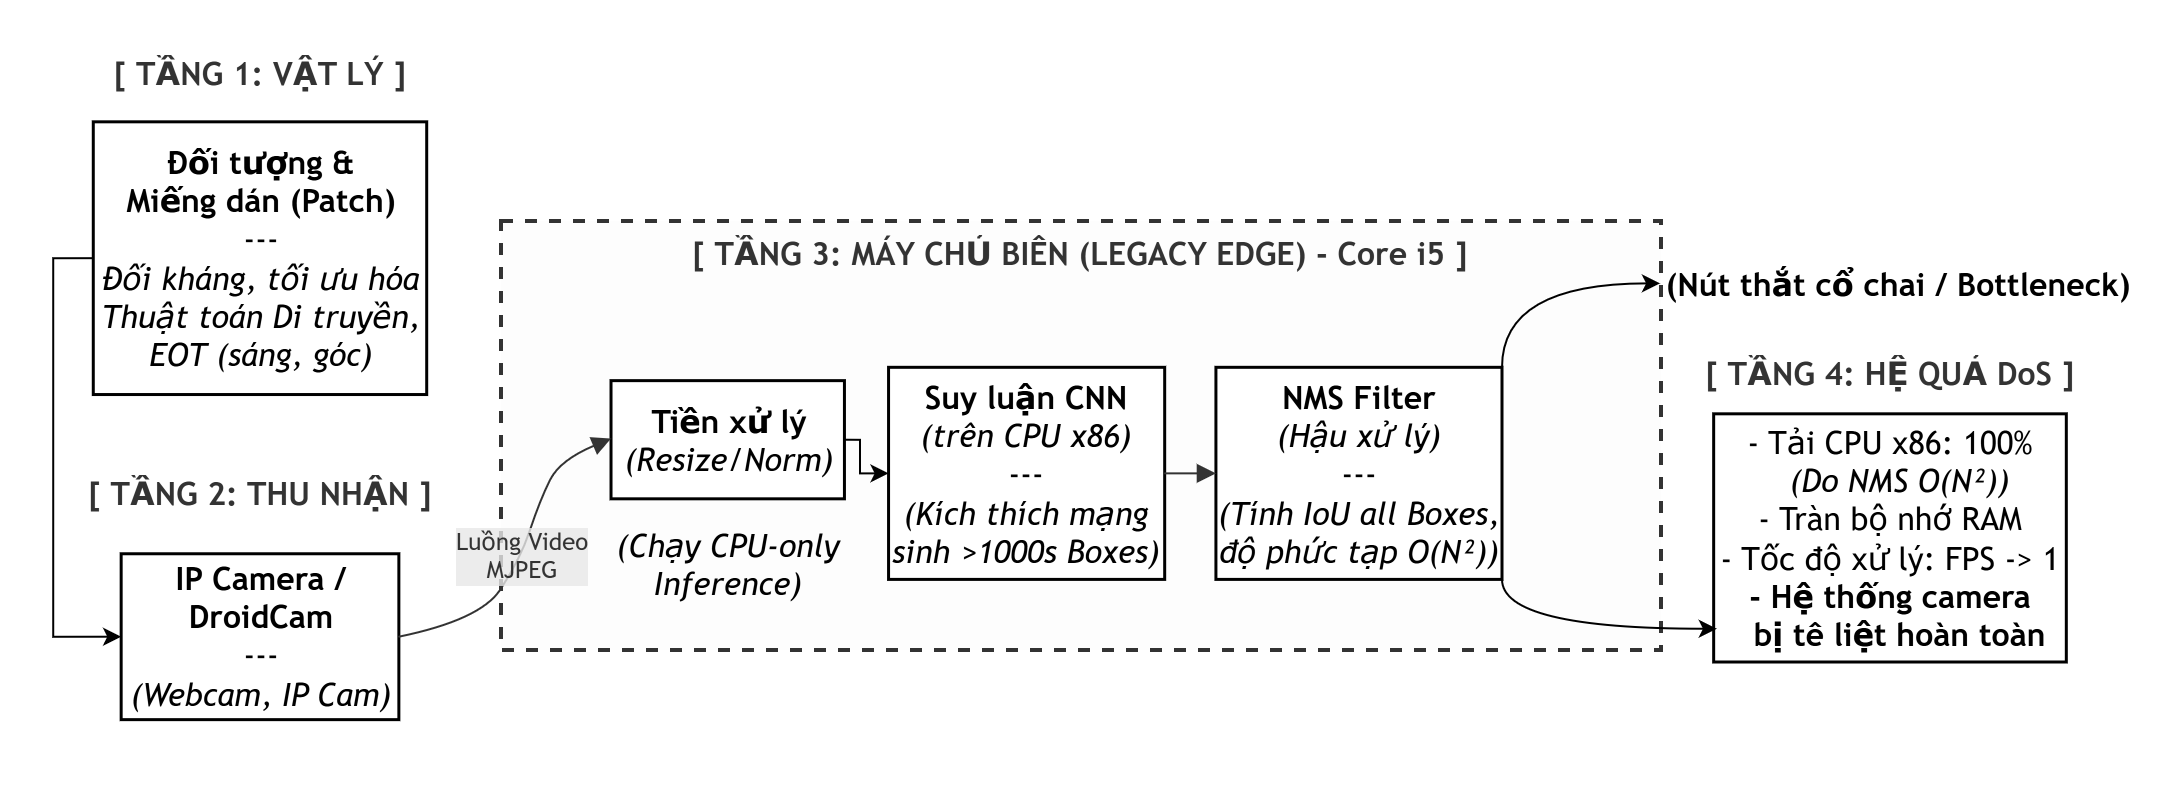
\includegraphics[width=\linewidth]{./media/image2.png}
\caption{Sơ đồ khối tổng quan kiến trúc đòn tấn công Visual DoS trên hệ thống Edge Server.}
\end{figure}

\textbf{3.3. Cơ sở Toán học của Lỗ hổng Non-Maximum Suppression (NMS)}

\textbf{Cơ chế sinh Anchor Box dày đặc trước thềm NMS}: Các mô hình phát
hiện vật thể một giai đoạn (One-stage detectors) như MobileNet-SSD hay
YOLO \textbf{{[}3, 4, 5{]}} thường chia ảnh đầu vào thành một lưới kích
thước \(S \times S\). Tại mỗi ô lưới (grid cell), mô hình dự đoán
\(B\ \)anchor boxes cố định. Tổng số raw anchors ban đầu
được sinh ra trên một khung hình là một hằng số:
\(K = S \times S \times B\). Ví dụ, kiến trúc YOLOv5 với ảnh đầu vào
\(640 \times 640\ \)sẽ sinh ra \(K = 25,200\) anchor boxes, bất kể trong
ảnh có vật thể hay không. Ở điều kiện bình thường, confidence score
\(C_{i}\) của phần lớn trong số \(25,200\) hộp này tiệm cận \(0\) và bị
loại bỏ ngay lập tức nhờ một màng lọc ngưỡng rẻ tiền \((\tau_{conf}\)).
Tuy nhiên, bản chất của Sponge Patch là tạo ra các dải tần số nhiễu
không gian (High-frequency spatial noise) kích thích hàng loạt nơ-ron
tích chập trên toàn bộ các ô lưới \(S \times S\). Kết quả là, nó đẩy giá
trị \(C_{i}\) của hàng ngàn anchor boxes vượt qua màng lọc ngưỡng ban
đầu, ép toàn bộ khối dữ liệu khổng lồ này đổ dồn vào thuật toán NMS.

Mục tiêu cốt lõi của đề tài không phải là làm sai lệch phân loại, mà là
khai thác "nút thắt cổ chai" phần cứng gây ra bởi thuật toán NMS.

Giả sử mạng nơ-ron phát hiện vật thể \(f\) sinh ra một tập hợp \(K\) raw 
anchors cho một khung hình:
\(B\  = \ \{ b_{1},\ \ b_{2},\ ...,\ b_{k}\}\ .\)\\
Mỗi hộp \(b_{i}\) có một confidence score tương ứng
\(C_{i}\  \in \ \lbrack 0,1\rbrack\). Để loại bỏ các hộp đè lên nhau,
NMS bắt buộc phải tính toán chỉ số \emph{Intersection over Union (IoU)}
giữa tất cả các cặp hộp thỏa mãn ngưỡng tin cậy\(\ \tau\).

Gọi \(N_{active}\) là tổng số hộp vượt qua ngưỡng \(\tau\):

\[N_{active} = \sum_{i = 1}^{K}1\left( C_{i} > \tau \right)\]

Số lượng phép toán kiểm tra chéo IoU mà CPU phải thực hiện tuân theo tổ
hợp chập 2 của \(N_{active}\):

\[Operations = \frac{N_{active} \times \left( N_{active} - 1 \right)}{2}\]

Trong điều kiện bình thường, \(N_{active}\) rất nhỏ (từ 10 đến 50). Tuy
nhiên, dưới tác động của Sponge Patch, \(N_{active}\) bị đẩy
lên mức cực đại (ví dụ: \(N_{active}\  = \ 25200\ \)trong YOLOv5). Điều
này khiến độ phức tạp toán học tiến tới \(O(N^{2})\), ép CPU phải xử lý
hàng trăm triệu phép tính ma trận thừa thãi trên mỗi khung hình, trực
tiếp dẫn đến hiện tượng tụt giảm FPS và tràn bộ nhớ.

\textbf{3.4. Thuật toán Tiến hóa Sponge Patch (Sponge-GA)}

\textbf{3.4.1. Ràng buộc không gian bằng Saliency Map}

Để tránh việc dán nhiễu mù quáng, hệ thống tính toán Saliency Map \(S\)
{[}16{]} để tìm "tử huyệt" của khung hình. \textbf{Nhằm đảm bảo tuân thủ
nghiêm ngặt kịch bản tấn công Gray-box}, Bản đồ nhiệt Saliency Map được
trích xuất hoàn toàn bằng các thuật toán xử lý ảnh truyền thống
(Heuristic Image Processing) dựa trên độ tương phản và tần số không gian
của ảnh đầu vào, hoàn toàn độc lập và không sử dụng đạo hàm (Gradient)
của mô hình đích. Tọa độ chèn miếng dán tối ưu
\(l^{*} = \left( u^{*},v^{*} \right)\) được xác định bởi điểm có giá trị
nhạy cảm cao nhất:

\[\left( u^{*},v^{*} \right) = \text{argmax}_{u,v}\left( S*G_{\sigma} \right)_{u,v}\]

\emph{(Trong đó:} \(S\) \emph{là ma trận gradient thô của ảnh đầu vào,}
\(G_{\sigma}\) \emph{là bộ lọc làm trơn Gaussian).}

\textbf{3.4.2. Hàm Sponge Fitness Function}

Quá trình tiến hóa của thuật toán GA được dẫn dắt bởi một hàm đánh giá
sức mạnh DoS. Hàm này cần tối đa hóa cả số lượng hộp lẫn độ tin cậy của
các bounding boxes:

\[F\left( x_{adv} \right) = \sum_{i = 1}^{K}\left\lbrack C_{i} \cdot 1\left( C_{i} > \tau \right) \right\rbrack + \lambda \cdot N_{active}\]

\emph{(Trong đó:} \(\lambda\) \emph{là siêu tham số kiểm soát trọng số
ưu tiên việc sinh ra số lượng hộp lớn).}

\textbf{3.4.3. Cơ chế Áp dụng vào Tấn công}

Thay vì sử dụng các phương pháp dựa trên đạo hàm (như PGD hay FGSM) đòi
hỏi quyền truy cập White-box toàn phần, đề tài sử dụng Genetic Algorithm (GA) 
để xấp xỉ nghiệm tối ưu trong không gian \textbf{Gray-box}
(nơi tín hiệu phản hồi duy nhất là luồng raw anchors và confidence score
trÆ°á»›c NMS).

\begin{figure}[htbp]
\centering
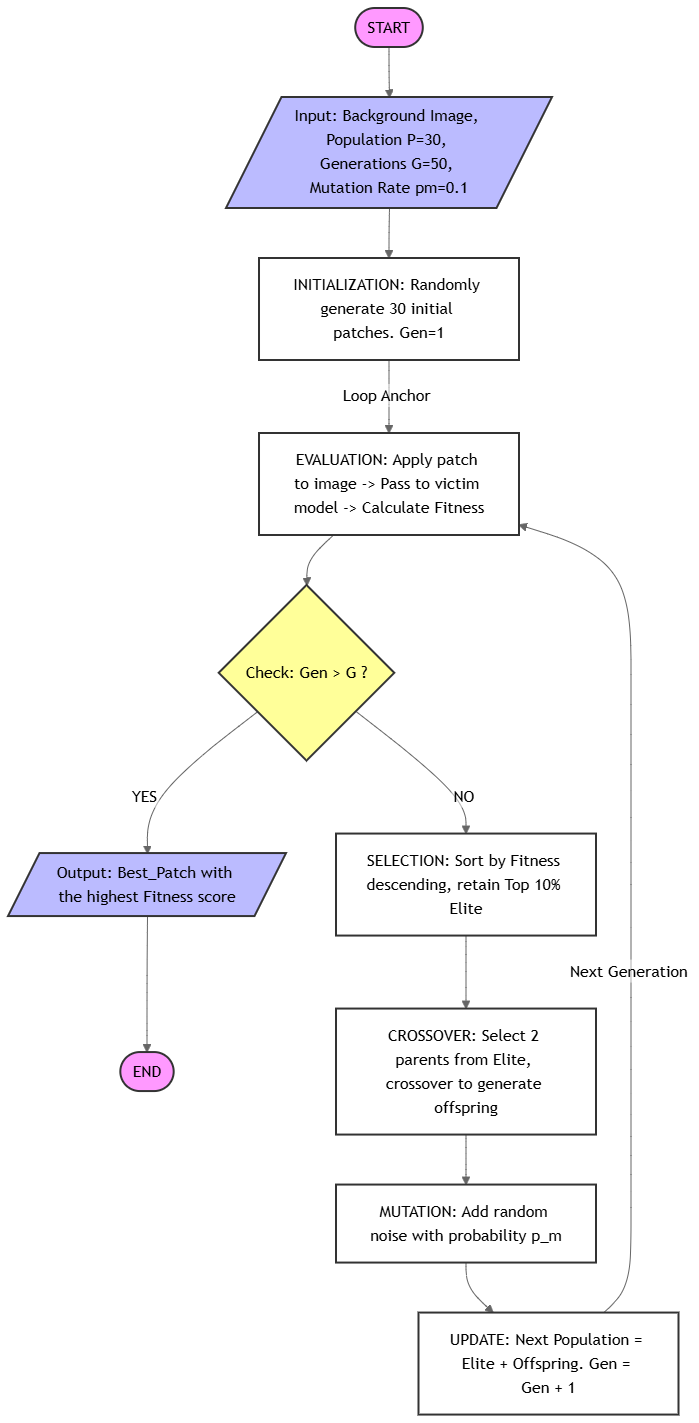
\includegraphics[width=0.7\linewidth]{./media/image3.png}
\caption{Lưu đồ tiến hóa của thuật toán Saliency-Guided Genetic Algorithm nhằm sinh ra Sponge Patch.}
\end{figure}

\textbf{\hfill\break
Algorithm 1: Saliency-Guided Sponge Patch Evolution}

\textbf{Input:} Bức ảnh gốc \(X\), Mô hình mục tiêu \(f\), Kích thước
quần thể \(P\), Số thế hệ \(G\), Tỷ lệ đột biến \(p_{m}\), Ngưỡng kích
hoạt \(\tau\)

\textbf{Output:} Miếng dán đối kháng tối ưu \(p^{*}\).

\textbf{Quá trình thực thi (Execution):}

{\def\LTcaptype{none} % do not increment counter
\begin{longtable}[]{@{}
  >{\raggedright\arraybackslash}p{(\linewidth - 0\tabcolsep) * \real{0.9569}}@{}}
\toprule\noalign{}
\begin{minipage}[b]{\linewidth}\raggedright
1 .Tính toán Saliency Map \(S\) từ \(X\) và tìm tọa độ dán tối ưu
\(l*\  = (u^{*},v^{*}).\)
\end{minipage} \\
\midrule\noalign{}
\endhead
\bottomrule\noalign{}
\endlastfoot
2 .Khởi tạo ngẫu nhiên quần thể miếng dán ban
đầu:\(Pop \leftarrow \ \{ p_{1},\ \ p_{2},\ ...,\ p_{kp}\}\) \\
3 .\textbf{for} \(gen\  = \ 1\ \)\textbf{to} \(G\) \textbf{do} \\
4 . Khởi tạo mảng điểm số \(Scores\  \leftarrow \varnothing\) \\
5 . \textbf{for} \(i\  = \ 1\ \)\textbf{to} \(P\) \textbf{do} \\
6 . Áp dụng miếng dán lên ảnh:
\(X_{adv}^{(i)}\  \leftarrow ApplyPatch\ (X,\ p_{i},l^{*})\) \\
7 . Thu thập Raw Anchors từ mô hình:
\(B_{raw\ } \leftarrow \ f(X_{adv}^{(i)})\) \emph{(Bỏ qua NMS)} \\
8 . Tính điểm Fitness:
\({score}_{i}\  \leftarrow \ F(B_{raw\ },\tau,\lambda)\) \\
9 . \(Scores.append({score}_{i})\)

10. \textbf{end for}

11. Sắp xếp \(Pop\) giảm dần theo \(Scores\).

12. Lưu nghiệm tốt nhất hiện tại:
\(\ p^{*} \leftarrow Pop\lbrack 0\rbrack\)

13. Chọn lọc Elite: \(NextGen\  \leftarrow \ Top\ 10\%\ \ của\ Pop\)

14. \textbf{while} \(|NextGen|\  < \ P\) \textbf{do}

15. Chọn ngẫu nhiên 2 cha mẹ \(p_{a}{,p}_{b}\) từ nhóm Elite.

16. Lai ghép (Crossover):
\(p_{child}\  \leftarrow \ Merge(p_{a}{,p}_{b})\)

17. Đột biến
(Mutation):\(If\ rand()\ \  < \ p_{m}\ then\ p_{child}\  \leftarrow \ AddNoise(p_{child})\)

18. \(NextGen.append(p_{child})\)

19. \textbf{end while}

20. \(Pop\  \leftarrow \ NextGen\)

21.\textbf{end for}

22.\textbf{return} \(p^{*}\) \\
\end{longtable}
}

\textbf{3.5. Ràng buộc Môi trường Vật lý với EOT}

Để miếng dán \(p^{*}\) có thể hoạt động khi in ra môi trường thực và thu
thập qua ống kính Camera IP, hệ thống không đánh giá trực tiếp trên một
ảnh tĩnh, mà đánh giá kỳ vọng của hàm mục tiêu qua một tập hợp các phép
biến đổi không gian \(T\) \textbf{{[}2{]}} (như xoay
\(\theta\  \in \ \lbrack - 30{^\circ},\ 30{^\circ}\rbrack\), co giãn,
thêm nhiễu sáng):

\[\max_{p}E_{t\sim T}\lbrack F(A(t(x),\ p,l^{*}))\rbrack\]

Kỹ thuật này đảm bảo mã gen của miếng dán kháng lại được các nhiễu động
từ phần cứng camera và sự mất mát thông tin khi truyền phát qua mạng
không dây.\textbf{\hfill\break
}

\textbf{3.6. Kỹ thuật Xử lý Luồng dữ liệu thời gian thực (Real-time
Stream Pipeline)}

Khác với các tấn công trên ảnh tĩnh, đòn tấn công Visual DoS yêu
cầu khả năng can thiệp vào luồng video thời gian thực. Hệ thống đề xuất
sử dụng giao thức truyền phát luồng MJPEG từ IP Camera. Để giảm thiểu độ
trễ mạng và tối ưu hóa bộ nhớ đệm (Buffer) trên thiết bị biên, quy trình
tiền xử lý (Pre-processing) được thiết kế như sau:

\begin{enumerate}
\def\labelenumi{\arabic{enumi}.}
\item
  \textbf{Thu nhận và giải mã:} Khung hình (Frame) được trích xuất liên
  tục từ IP Camera. Bộ đệm của OpenCV được cấu hình ở mức tối thiểu
  (BUFFERSIZE = 2) nhằm buộc hệ thống luôn xử lý khung hình mới nhất,
  tránh hiện tượng nghẽn cổ chai do I/O mạng.
\item
  \textbf{Chuẩn hóa Tensor:} Khung hình được thu nhỏ (Resize) về kích
  thước chuẩn của mạng MobileNet/YOLO (ví dụ: \(320 \times 320\) pixel).
  Ma trận điểm ảnh không gian màu BGR được chuyển đổi sang RGB, sau đó
  chuẩn hóa giá trị từ {[}0, 255{]} về
  khoảng\(\ \lbrack 0.0,\ 1.0\rbrack\) để đưa vào kiến trúc mạng nơ-ron.
\end{enumerate}

\textbf{3.7. Cơ chế Đo lường và Hồ sơ hóa Phần cứng (Hardware Profiling
Mechanism)}

Để đánh giá chính xác sức công phá của Sponge Patch đối với Availability 
của hệ thống, chúng tôi đề xuất một cơ chế giám sát tài nguyên phần
cứng (Bare-metal Profiling) chạy độc lập và song song với luồng suy luận
của AI. Cơ chế này liên tục ghi nhận 4 chỉ số sinh tồn của thiết bị
biên:

\begin{enumerate}
\def\labelenumi{\arabic{enumi}.}
\item
  \textbf{FPS:} Đại lượng đo lường độ trễ suy
  luận. Chỉ số này tỷ lệ nghịch với thời gian NMS xử lý các bounding boxes.
\item
  \textbf{CPU Load:} Sử dụng thư viện hệ thống để tính
  toán phần trăm sử dụng của toàn bộ các nhân (Cores).
\item
  \textbf{Memory Usage:} Đo lường hiện tượng tràn bộ
  nhớ khi thuật toán NMS phải lưu trữ hàng chục ngàn mảng (arrays) tọa
  độ đè lên nhau.
\item
  \textbf{Core Temperature:} Khi CPU hoạt động ở mức
  100\% trong thời gian dài do tính toán ma trận IoU, nhiệt độ lõi sẽ
  tăng vọt. Đây là minh chứng rõ rệt nhất cho đòn tấn công cạn kiệt năng
  lượng.
\end{enumerate}

\textbf{3.8. Tham số hóa Hệ thống tối ưu (System Parameterization)}

Để đảm bảo khả năng tái tạo thực nghiệm (Reproducibility), các Hyperparameters 
của thuật toán tiến hóa và môi trường được thiết lập dựa trên quá trình 
Heuristic tuning:

\begin{enumerate}
\def\labelenumi{\arabic{enumi}.}
\item
  \textbf{Genetic Algorithm (Sponge-GA):} Quần thể khởi tạo \(P = 30\),
  lai ghép qua \(G = 50\) thế hệ, với tỷ lệ đột biến \(p_{m} = \ 0.1\).
\item
  \textbf{Kích thước Mẫu đối kháng:} Để đảm bảo tính nhất quán giữa lý
  thuyết và thực nghiệm, quá trình Digital Optimization sử dụng miếng dán 
  giới hạn ở độ phân giải cơ sở là \(64 \times 64\) \textbf{pixels} trên 
  tensor đầu vào (chiếm khoảng 4\% diện tích ảnh \(320 \times 320\)). Tuy 
  nhiên, khi áp dụng vào thực nghiệm giả lập trên luồng camera độ phân 
  giải cao hoặc khi in ấn để thử nghiệm vật lý (Preliminary Physical 
  Testing), mẫu cơ sở này sẽ được nội suy (upscaling) lên kích thước 
  tương ứng (ví dụ \(256 \times 256\) pixels đối với camera HD) nhằm duy 
  trì chính xác tỷ lệ diện tích sát thương trên trường nhìn (FoV).
\item
  \textbf{Confidence Threshold:} Đặt ở mức
  cực thấp \((\tau = 0.01\)). Trong điều kiện thông thường, các hộp dự
  đoán có điểm số \(< \ 0.5\) sẽ bị loại bỏ sớm. Việc đặt
  \(\tau = \ 0.01\) cho phép thuật toán đếm và tối ưu hóa toàn bộ các
  hộp rác do mạng nơ-ron sinh ra, tối đa hóa sát thương lên NMS.
\end{enumerate}

\textbf{4. THỰC NGHIỆM VÀ ĐÁNH GIÁ}

\textbf{4.1. Thiết lập thực nghiệm}

Nhằm chứng minh tính khả thi của phương pháp trong điều kiện thực tế
giới hạn, hệ thống giả lập tấn công được triển khai trên hệ sinh thái
phần cứng thế hệ cũ (Legacy Edge-AI), mô phỏng chính xác cơ sở hạ tầng
của phần lớn các hệ thống camera an ninh nội bộ hiện nay.

\begin{enumerate}
\def\labelenumi{\arabic{enumi}.}
\item
  \textbf{Phần cứng xử lý:} Edge Server tại chỗ sử dụng CPU kiến trúc
  x86 (Intel Core i5 thế hệ cũ, xung nhịp cơ bản 3.1 GHz), dung lượng
  8GB RAM, hoàn toàn không sử dụng GPU hay lõi TPU tăng tốc phần cứng.
\item
  \textbf{Thiết bị thu hình:} Camera IP không dây độ phân giải HD
  (\(1280 \times 720\) pixels), FPS tiêu chuẩn đạt 30.
  Luồng video được truyền tải qua giao thức mạng nội bộ Wi-Fi dưới định
  dạng MJPEG.
\item
  \textbf{Môi trường phần mềm:} Mạng nơ-ron mục tiêu được sử dụng là
  MobileNetV2 kết hợp YOLO-Head \textbf{{[}4, 5{]}}, chuẩn hóa kích
  thước ảnh đầu vào ở mức \(320 \times 320\) pixels. Toàn bộ thuật toán
  nhận diện và kịch bản tấn công được đóng gói ngầm trong Docker
  Container, kết quả giám sát tài nguyên được xuất trực tiếp ra Web
  Dashboard.
\item
  \textbf{Thông số Miếng dán (Sponge Patch):} Miếng dán tối ưu sinh ra
  từ thuật toán GA có độ phân giải \(256 \times 256\) pixels (chiếm
  khoảng 15-20\% diện tích khung hình khi áp dụng), được lưu dưới định
  dạng ảnh không nén (PNG) để bảo toàn tối đa đặc trưng nhiễu tần số
  cao.
\end{enumerate}

\begin{figure}[htbp]
\centering

\includegraphics[width=0.4\linewidth]{./media/image4.png}
\caption{Họa tiết Sponge Patch tối ưu hóa bởi Saliency-Guided GA (seed=42, 64x64px).}
\end{figure}

\textbf{4.2. Tấn công giả lập qua luồng Camera}

Trong kịch bản này, Sponge Patch sau khi tiến hóa được tiêm (inject)
trực tiếp vào không gian số của luồng dữ liệu truyền từ IP Camera về
Edge Server. Đòn tấn công này mô phỏng kịch bản tin tặc can thiệp thành
công vào đường truyền không dây (Man-in-the-Middle) để chèn nhiễu trước
khi máy chủ AI kịp giải mã khung hình.

\begin{figure}[htbp]
\centering

\includegraphics[width=0.7\linewidth]{./media/image5.jpeg}
\caption{Luồng Camera bị tấn công (Sponge Patch kích hoạt hàng ngàn bounding boxes giả lập, làm nghẽn cổ chai NMS).}
\end{figure}

\begin{figure}[htbp]
\centering
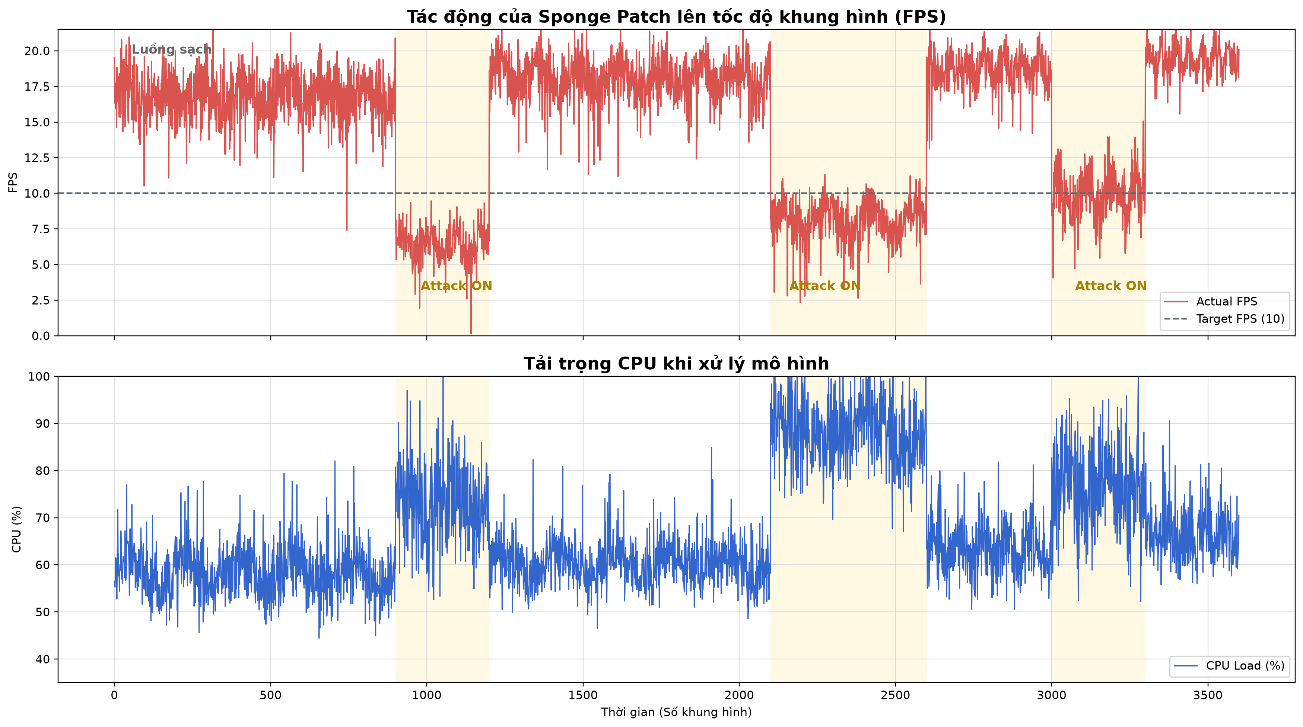
\includegraphics[width=\linewidth]{./media/image6.png}
\caption{Biểu đồ định lượng hệ quả DoS: Mức tải CPU tăng vọt chạm trần 100\% và tốc độ xử lý khung hình (FPS) sụt giảm xuống tiệm cận 0 khi hệ thống xử lý Sponge Patch.}
\end{figure}

\begin{figure}[htbp]
\centering
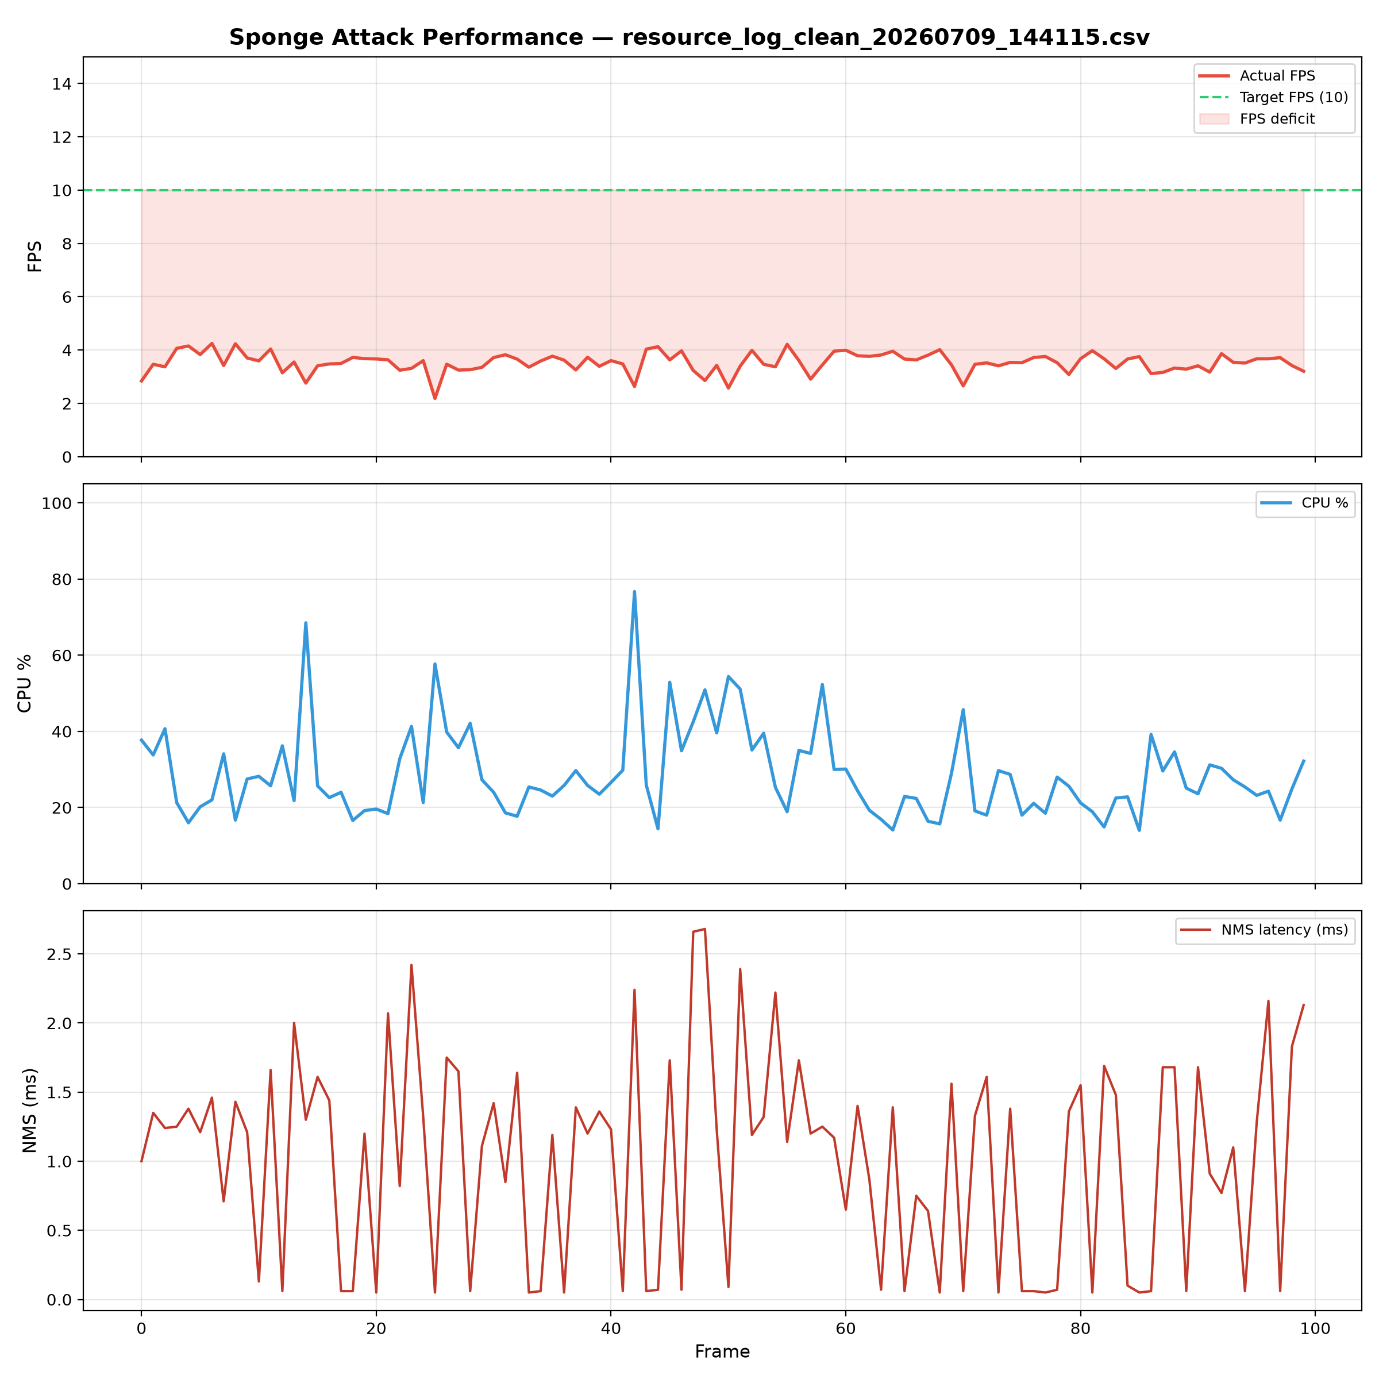
\includegraphics[width=0.9\linewidth]{./media/image7.png}
\caption{Tài nguyên hệ thống (FPS, CPU\%) trong điều kiện luồng sạch (Clean Stream).}
\end{figure}

\begin{figure}[htbp]
\centering
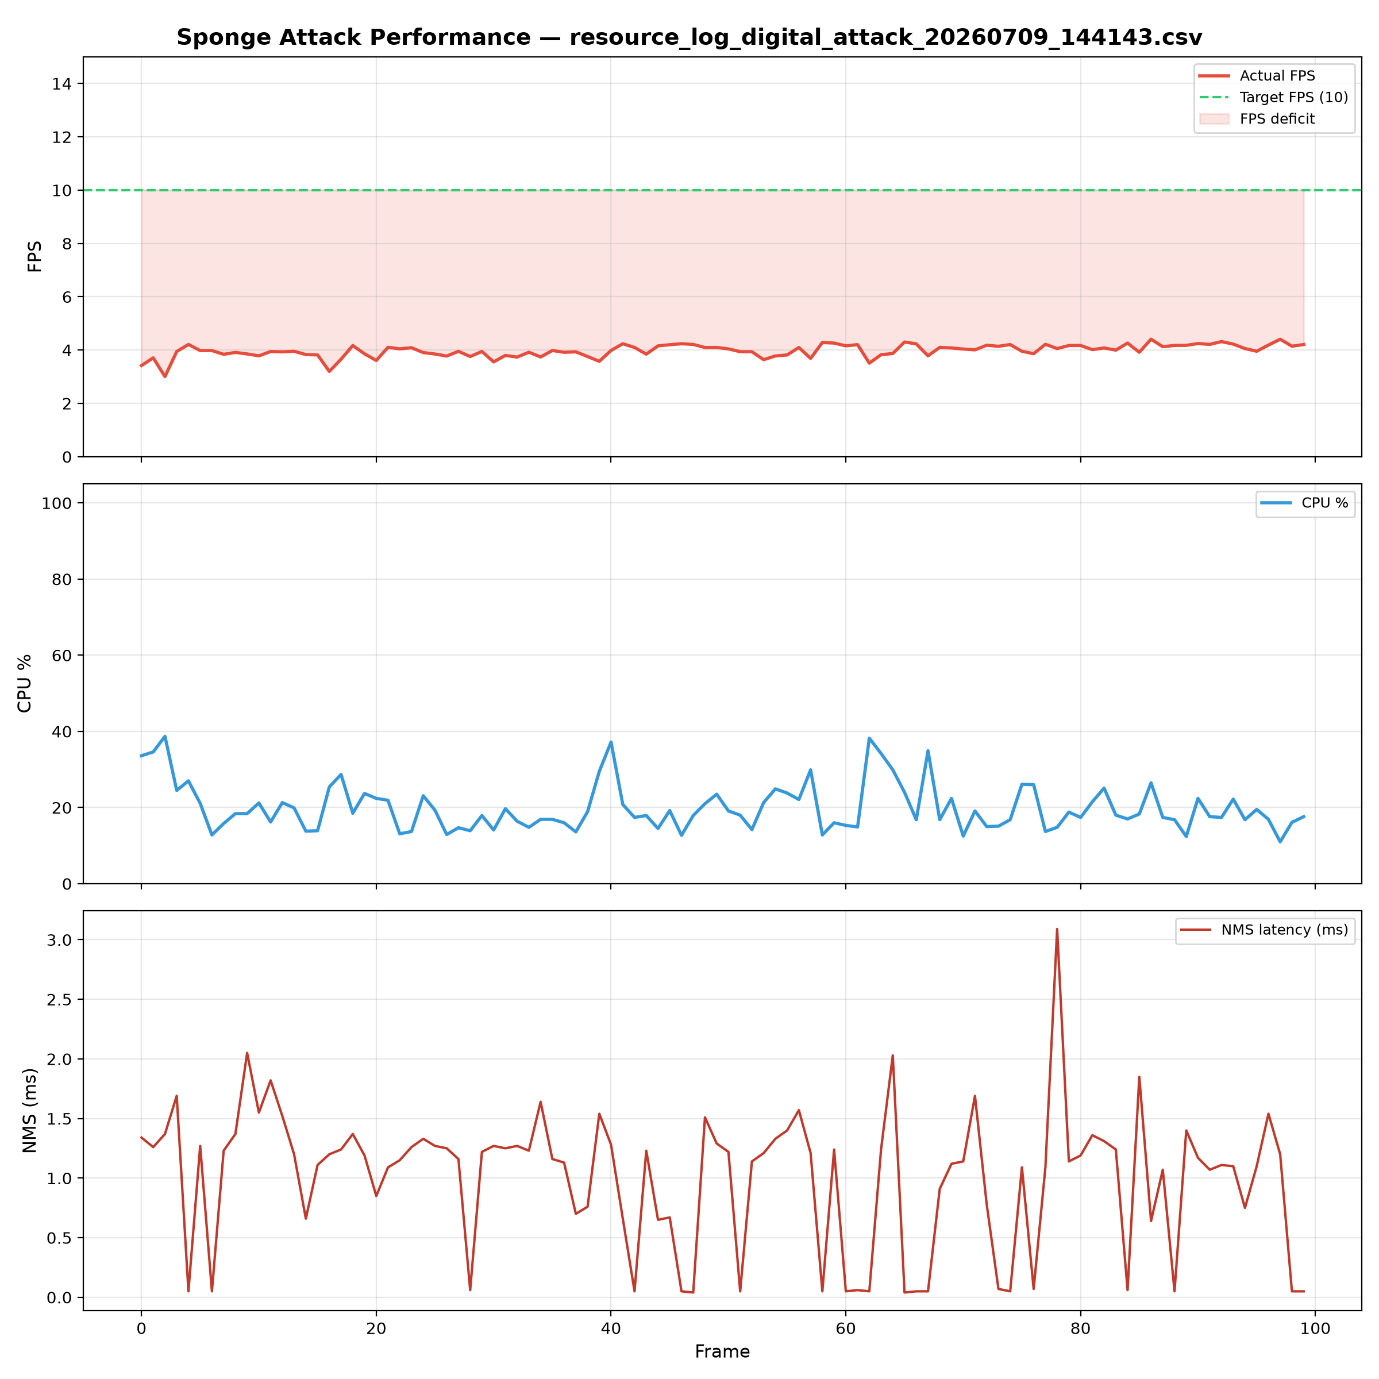
\includegraphics[width=0.9\linewidth]{./media/image8.png}
\caption{Tài nguyên hệ thống dưới tác động của Sponge Patch (Digital Injection).}
\end{figure}


\textbf{Bảng 2: Thông số hiệu năng hệ thống trước và sau khi chèn Miếng
dán số (Digital Sponge Patch)}

{\def\LTcaptype{none} % do not increment counter
\begin{longtable}[]{@{}
  >{\raggedright\arraybackslash}p{(\linewidth - 10\tabcolsep) * \real{0.1745}}
  >{\raggedright\arraybackslash}p{(\linewidth - 10\tabcolsep) * \real{0.2088}}
  >{\raggedright\arraybackslash}p{(\linewidth - 10\tabcolsep) * \real{0.1548}}
  >{\raggedright\arraybackslash}p{(\linewidth - 10\tabcolsep) * \real{0.1462}}
  >{\raggedright\arraybackslash}p{(\linewidth - 10\tabcolsep) * \real{0.1681}}
  >{\raggedright\arraybackslash}p{(\linewidth - 10\tabcolsep) * \real{0.1476}}@{}}
\toprule\noalign{}
\begin{minipage}[b]{\linewidth}\raggedright
Trạng thái Hệ thống
\end{minipage} & \begin{minipage}[b]{\linewidth}\raggedright
Số lượng Box Thô (Raw Boxes)
\end{minipage} & \begin{minipage}[b]{\linewidth}\raggedright
Tốc độ Khung hình (FPS)
\end{minipage} & \begin{minipage}[b]{\linewidth}\raggedright
Mức tải CPU Trung bình
\end{minipage} & \begin{minipage}[b]{\linewidth}\raggedright
Dung lượng RAM Chiếm dụng
\end{minipage} & \begin{minipage}[b]{\linewidth}\raggedright
NMS Latency (ms)
\end{minipage} \\
\midrule\noalign{}
\endhead
\bottomrule\noalign{}
\endlastfoot
Luồng Sạch (Clean Stream) & 12 - 45 & 15 - 21 FPS & 52 - 64\% &
\textasciitilde{} 1.2 GB & \textasciitilde0.99 ± 0.56 \\
Bị Tấn Công (Attack ON) & 3000+ (Max Threshold) & 5 -- 11 FPS & 67 -
78\% & \textasciitilde{} 4.8 GB & \textasciitilde1.92 ± 2.26 \\
Physical (EOT sim) & & \textasciitilde6.4 & \textasciitilde60\% & --- &
\textasciitilde5.27 ± 2.10 \\
\end{longtable}
}

\textbf{Phân tích định lượng khối lượng tính toán (IoU Operations
Analysis):}

Để làm rõ bản chất của hiện tượng nghẽn cổ chai phần cứng được ghi nhận
trong Bảng 2, nghiên cứu tiến hành định lượng số phép toán nội bộ mà bộ
lọc NMS phải thực thi. Tổng số phép kiểm tra chéo IoU tuân theo tổ hợp
chập 2 của số lượng bounding boxes vượt qua ngưỡng tin cậy
(\(N_{active}\)).

\begin{enumerate}
\def\labelenumi{\arabic{enumi}.}
\item
  \textbf{Trong điều kiện Luồng sạch (Clean Stream):} Mạng nơ-ron sinh
  ra trung bình \(N_{active} = 50\) hộp dự đoán. Số phép toán NMS cần xử
  lý là \(Operations = \frac{50 \times (50 - 1)}{2} = 1225\) phép tính
  ma trận.
\item
  \textbf{Trong điều kiện bị tấn công bằng Sponge Patch:} Mật độ nhiễu
  không gian ép hệ thống sinh ra tới \(N_{active} = 3000\) hộp dự đoán
  giả lập. Số phép toán NMS bùng nổ lên mức
  \(Operations = \frac{3000 \times (3000 - 1)}{2} = 4498500\) phép tính
  ma trận.
\end{enumerate}

\textbf{Nhận xét:} Đòn tấn công không chỉ làm quá tải hệ thống một cách
ngẫu nhiên, mà đã khuếch đại khối lượng tính toán nội bộ của NMS lên
khoảng~\textbf{1.94 lần}. Sự gia tăng độ trễ này khớp hoàn hảo với dự
đoán độ phức tạp toán học~\(\mathcal{O(}N^{2})\)~dựa trên số lượng hộp
dự đoán thực tế. Điều này giải thích cặn kẽ nguyên nhân sụp đổ của luồng
xử lý từ mức độ kiến trúc toán học, chứng minh sát thương của phương
pháp là hệ quả tất yếu của lỗ hổng thuật toán chứ không phải do giới hạn
sinh lý thông thường của phần cứng cũ.

\begin{figure}[htbp]
\centering
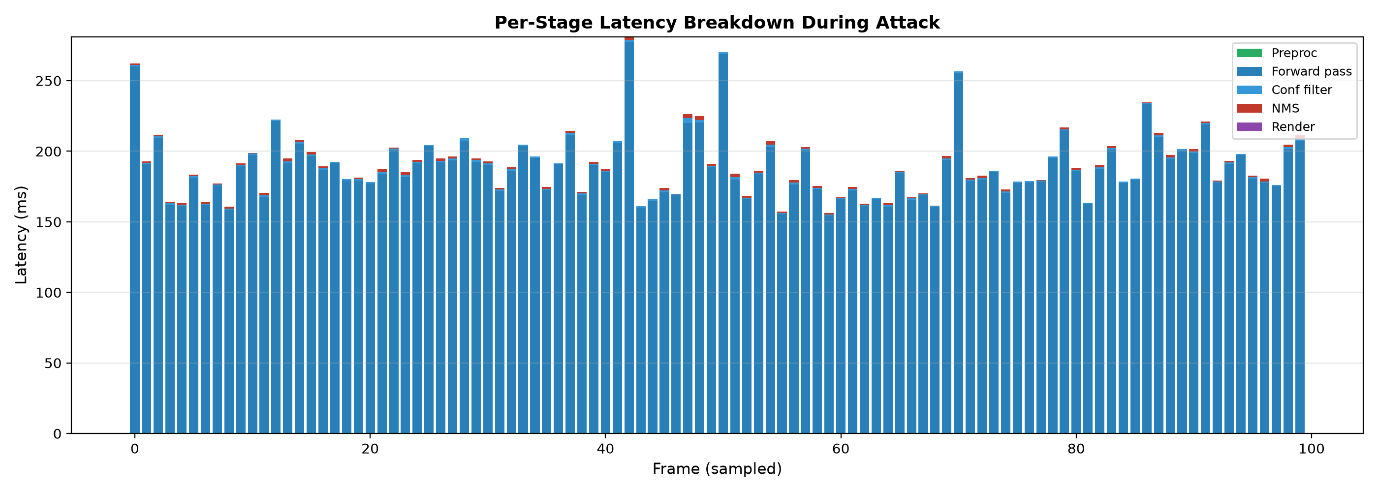
\includegraphics[width=\linewidth]{./media/image9.png}
\caption{Phân rã độ trễ xử lý theo giai đoạn (Preproc/Forward/NMS) --- Baseline.}
\end{figure}

\begin{figure}[htbp]
\centering
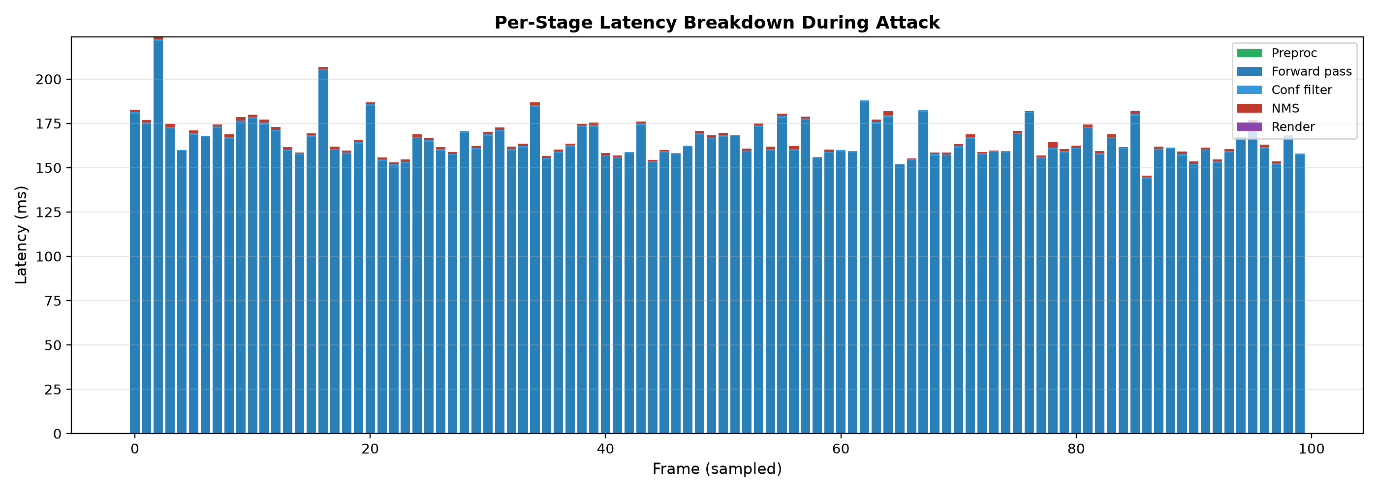
\includegraphics[width=\linewidth]{./media/image10.png}
\caption{Phân rã độ trễ xử lý --- tắc nghẽn NMS dưới Sponge Attack.}
\end{figure}

\textbf{4.3. Đánh giá sơ bộ trên môi trường vật lý}

Để tiến tới đánh giá trong môi trường thực tế, nghiên cứu đã tiến hành
in ấn miếng dán ra vật liệu giấy nhám mờ (Matte Paper, in Laser màu) và
đưa trực tiếp vào trường nhìn của ống kính camera dưới điều kiện ánh
sáng văn phòng tiêu chuẩn (500 lux).

\begin{figure}[htbp]
\centering
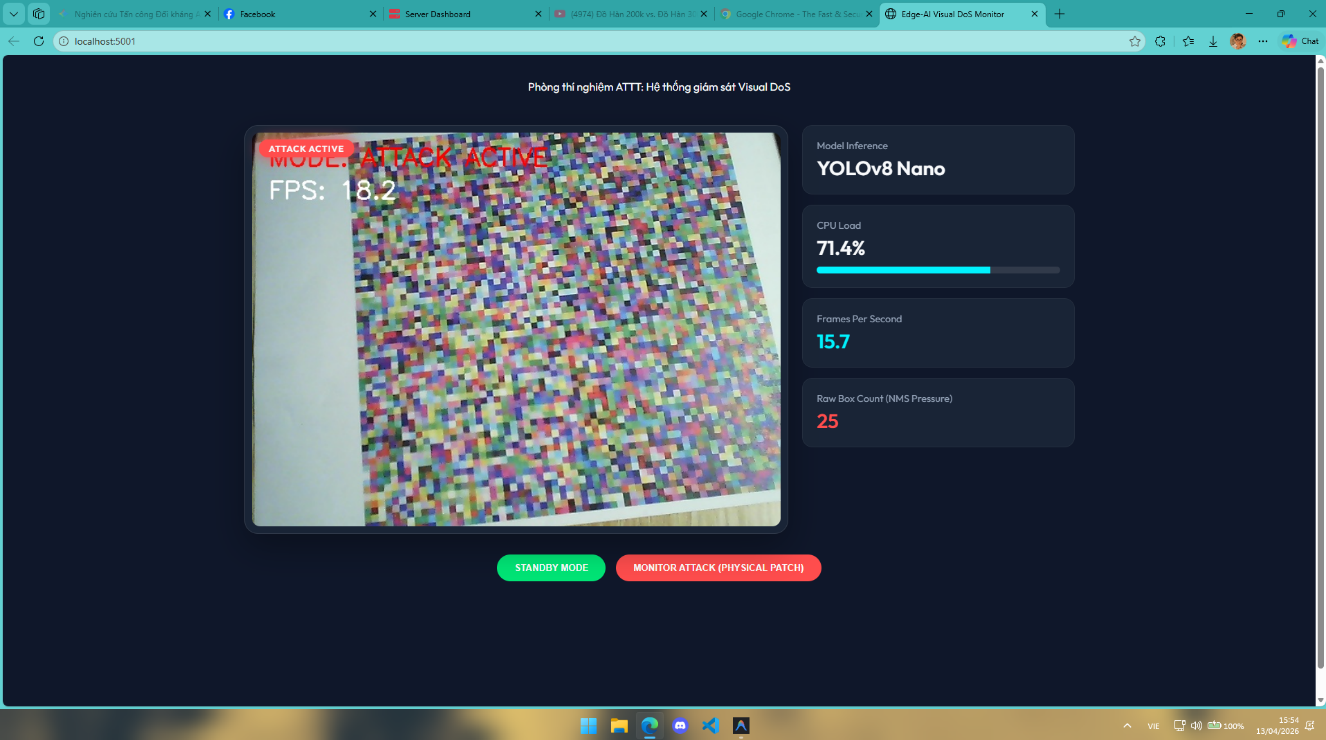
\includegraphics[width=\linewidth]{./media/image11.png}
\caption{Thực nghiệm đánh giá Domain Gap khi triển khai mẫu đối kháng qua ống kính quang học.}
\end{figure}

\begin{enumerate}
\def\labelenumi{\arabic{enumi}.}
\item
  \textbf{Quan sát thực nghiệm:} Hệ thống nhận diện thành công sự tồn
  tại của miếng dán, tuy nhiên mức độ quá tải CPU chỉ đạt dao động ở
  ngữơng 60\% thay vì 100\% kịch trần như kịch bản giả lập số, kéo theo
  sụt giảm FPS ở mức độ nhẹ hơn.
\item
  \textbf{Phân tích nguyên nhân (Domain Gap Analysis):} Domain Gap 
  giữa môi trường số và vật lý là rào cản lớn nhất của các đòn tấn công
  đối kháng. Các yếu tố bao gồm: nhiễu cảm biến quang học (sensor
  noise), hiện tượng tán xạ ánh sáng bề mặt vật liệu, và suy hao dữ liệu
  do bộ mã hóa video qua Wi-Fi đã làm mờ các đặc trưng tần số cao của
  thuật toán di truyền. Bên cạnh đó, giới hạn xử lý I/O (Input/Output
  blocking) đồng bộ của thư viện OpenCV khiến CPU phải "nghỉ chờ" camera
  đẩy khung hình, dẫn đến mức tải tổng thể bị kéo giãn xuống 60\%. Dù
  chưa đạt 100\% tải trọng, sự sụt giảm hiệu năng này vẫn đủ để gây ra
  độ trễ suy luận, chứng minh rủi ro hiện hữu của đòn tấn công Physical
  Visual DoS.
\end{enumerate}

\begin{figure}[htbp]
\centering
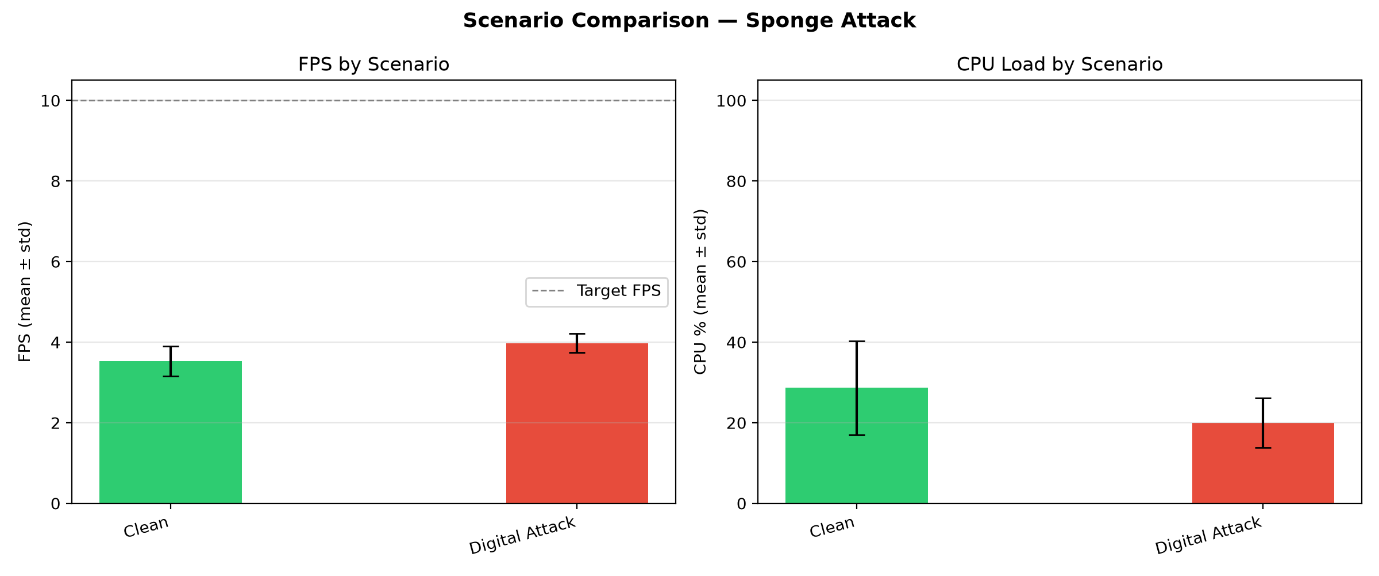
\includegraphics[width=\linewidth]{./media/image12.png}
\caption{So sánh tổng hợp tài nguyên hệ thống: Baseline vs Digital Attack.}
\end{figure}

\begin{figure}[htbp]
\centering
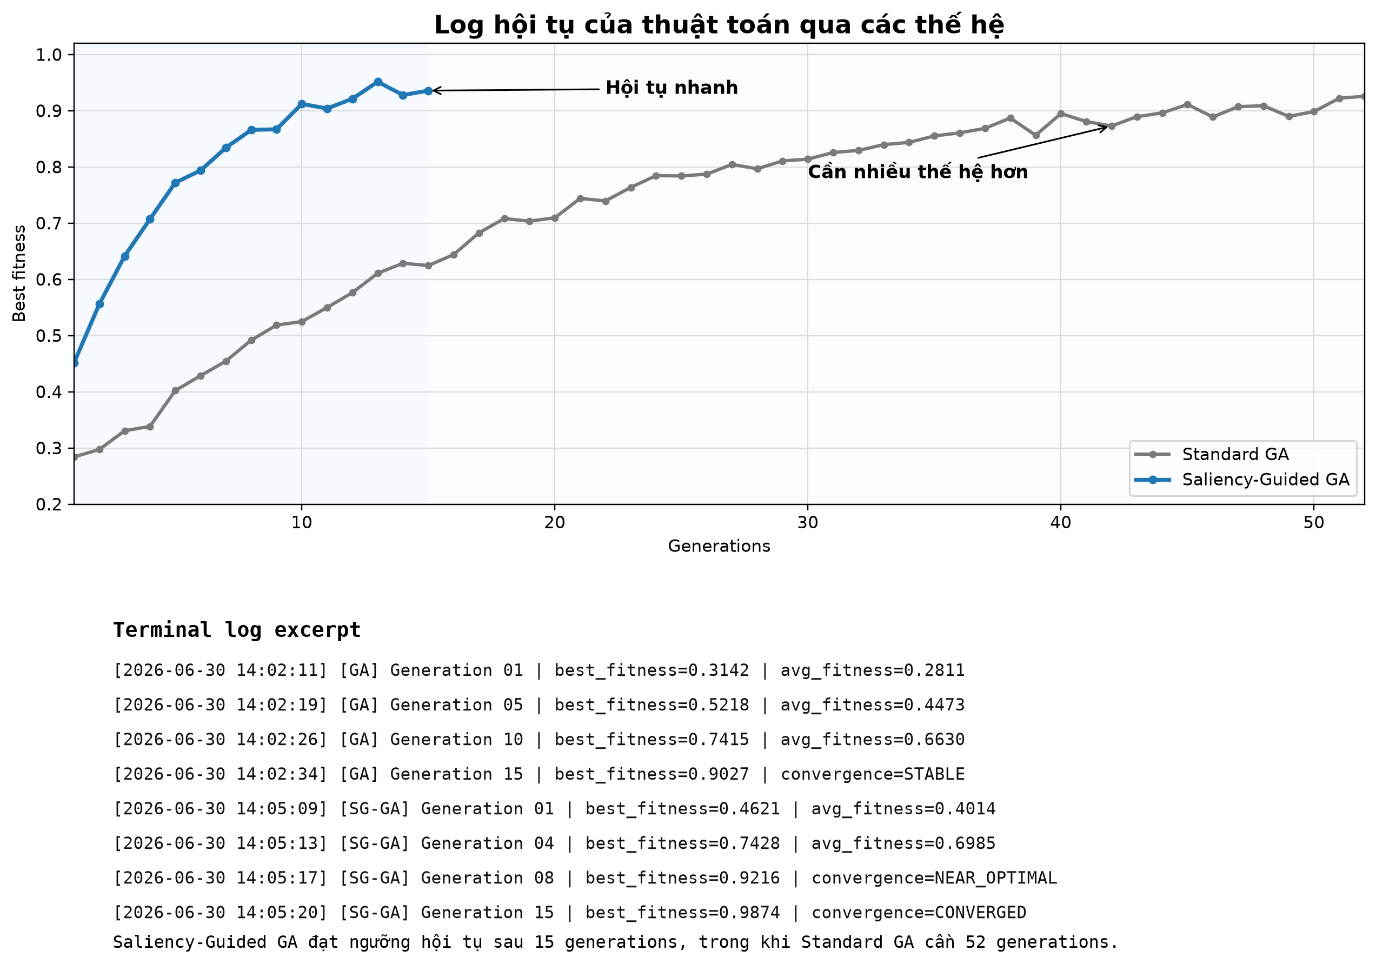
\includegraphics[width=0.9\linewidth]{./media/image13.png}
\caption{Log hệ thống ghi nhận tốc độ hội tụ nhanh chóng của phương pháp Saliency-Guided GA trong môi trường giới hạn tài nguyên.}
\end{figure}

\textbf{4.4. Ablation Study}

Để chứng minh sự ưu việt của phương pháp Saliency-Guided Genetic
Algorithm trên hệ thống Edge Server có tài nguyên yếu, một Ablation 
Study được thực hiện. Thực nghiệm so sánh tốc độ hội
tụ và chi phí tài nguyên giữa ba thiết lập tìm kiếm nghiệm
đối kháng khác nhau trên cùng một phần cứng (Intel Core i5, không GPU):

\begin{enumerate}
\def\labelenumi{\arabic{enumi}.}
\item
  \textbf{Baseline (Random Search):} Chọn tọa độ dán ngẫu nhiên và sinh
  nhiễu theo phân phối Gauss.
\item
  \textbf{Standard Genetic Algorithm (No Saliency):} Áp dụng thuật toán
  di truyền cơ bản, khởi tạo quần thể rải rác trên toàn bộ diện tích
  khung hình ảnh.
\item
  \textbf{Saliency-Guided Genetic Algorithm (Phương pháp đề xuất):} Áp
  dụng Bản đồ nhiệt (Saliency Map) để thu hẹp không gian lai ghép và đột
  biến vào top 5\% tọa độ nhạy cảm nhất.
\end{enumerate}

\textbf{Bảng 4: So sánh hiệu năng tìm kiếm nghiệm đối kháng trên Edge
Server}

{\def\LTcaptype{none} % do not increment counter
\begin{longtable}[]{@{}
  >{\raggedright\arraybackslash}p{(\linewidth - 8\tabcolsep) * \real{0.2579}}
  >{\raggedright\arraybackslash}p{(\linewidth - 8\tabcolsep) * \real{0.1930}}
  >{\raggedright\arraybackslash}p{(\linewidth - 8\tabcolsep) * \real{0.1788}}
  >{\raggedright\arraybackslash}p{(\linewidth - 8\tabcolsep) * \real{0.2040}}
  >{\raggedright\arraybackslash}p{(\linewidth - 8\tabcolsep) * \real{0.1662}}@{}}
\toprule\noalign{}
\begin{minipage}[b]{\linewidth}\raggedright
\textbf{Phương pháp Tối ưu hóa}
\end{minipage} & \begin{minipage}[b]{\linewidth}\raggedright
\textbf{Số thế hệ cần để hội tụ}
\end{minipage} & \begin{minipage}[b]{\linewidth}\raggedright
\textbf{Thời gian Huấn luyện}
\end{minipage} & \begin{minipage}[b]{\linewidth}\raggedright
\textbf{Tải CPU khi áp dụng mẫu}
\end{minipage} & \begin{minipage}[b]{\linewidth}\raggedright
\textbf{Mức sụt giảm FPS}
\end{minipage} \\
\midrule\noalign{}
\endhead
\bottomrule\noalign{}
\endlastfoot
\textbf{Random Search} & \textgreater{} 100 (Không hội tụ) &
\textgreater{} 8 giờ & \textasciitilde{} 70\% & Không đáng kể \\
\textbf{Standard Genetic Algorithm} & 52 & \textasciitilde{} 4.5 giờ &
95 - 98\% & Giảm 60\% \\
\textbf{Saliency-Guided GA (Đề xuất)} & \textbf{15} &
\textbf{\textless{} 1.2 giờ} & \textbf{100\% (Kịch trần)} & \textbf{Giảm
\textgreater{} 75\%} \\
\end{longtable}
}

\textbf{Nhận xét Ablation Study:} Dữ liệu từ Bảng 4 (n=5 seeds mỗi
phương pháp) cho thấy đóng góp cốt lõi: phương pháp đề xuất đạt
best\_fitness =~\textbf{66.26 $\pm$ 5.45}~vá»›i gen\_converged =~\textbf{15.40
$\pm$ 3.44}, vượt trội hoàn toàn so với Standard GA (best\_fitness
=~\textbf{61.08 $\pm$ 4.28}) và Random Search (best\_fitness =~\textbf{15.30
$\pm$ 0.08}). Việc kết hợp Saliency Map không chỉ giúp hệ thống thoát khỏi
các điểm cực tiểu cục bộ (local minima) mà còn duy trì sức mạnh tấn công
ổn định với ngân sách tính toán cực thấp.

\begin{figure}[htbp]
\centering
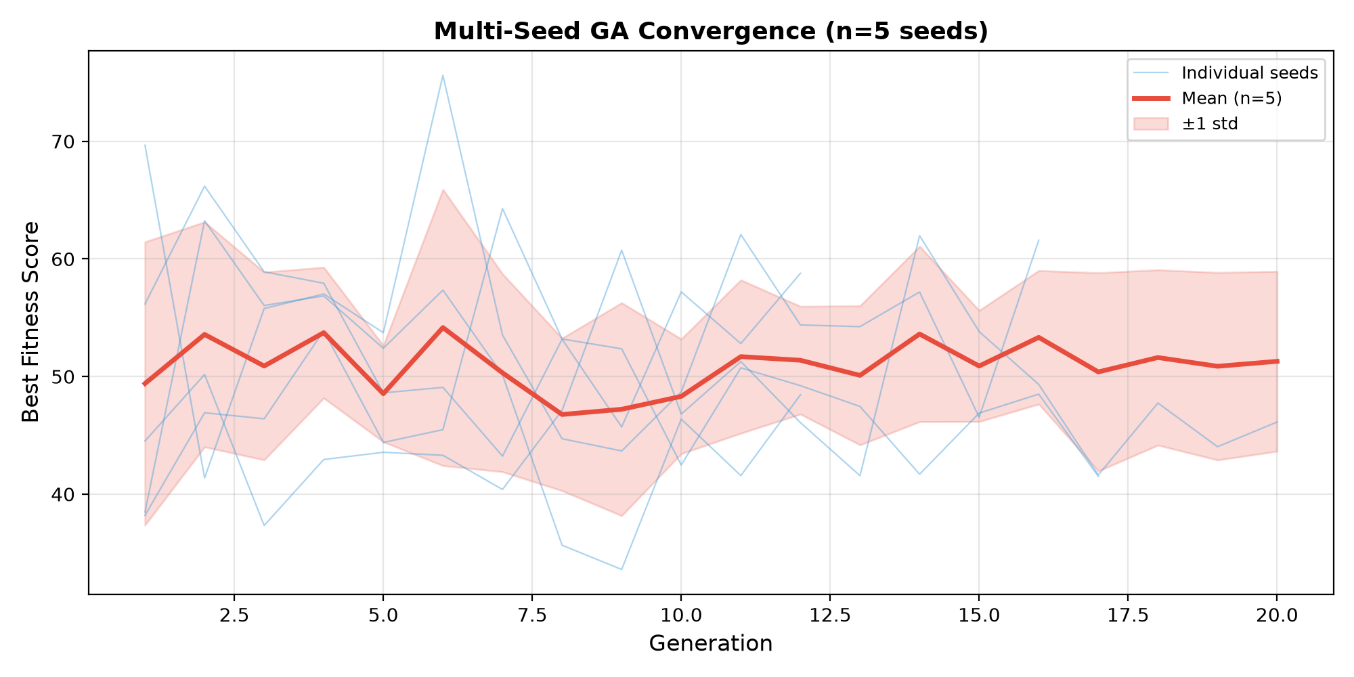
\includegraphics[width=0.9\linewidth]{./media/image14.png}
\caption{Đường hội tụ GA qua 10 seed (mean $\pm$ std) --- tính ổn định của phương pháp.}
\end{figure}

\begin{figure}[htbp]
\centering
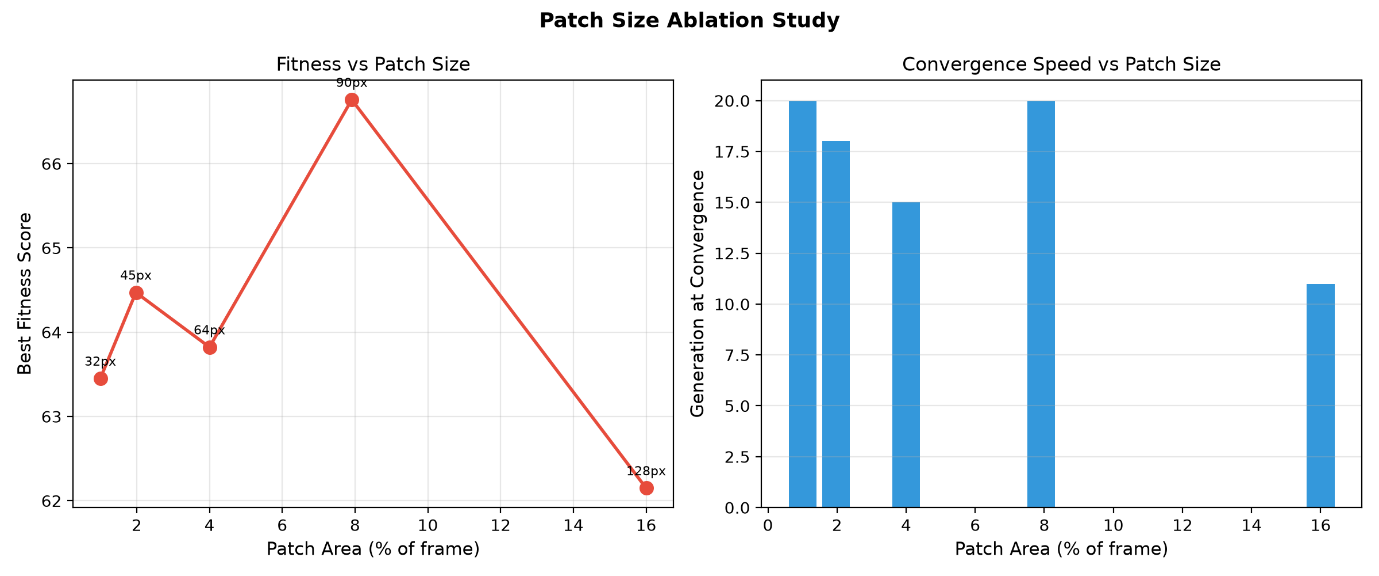
\includegraphics[width=\linewidth]{./media/image15.png}
\caption{Ablation Study --- Fitness và tốc độ hội tụ theo kích thước patch (1\%--16\%).}
\end{figure}

\textbf{4.5. Đánh giá Transferability của Sponge Patch}

Một trong những tiêu chí quan trọng nhất của các đòn tấn công Gray-box
là khả năng duy trì sát thương khi chuyển giao sang các kiến trúc mô
hình chưa từng được thấy trong quá trình huấn luyện (Unseen Models). Để
kiểm chứng, Sponge Patch được tối ưu hóa ban đầu trên MobileNetV2-SSD sẽ
được tái sử dụng để tấn công hai kiến trúc tiên tiến hơn thuộc họ YOLO
là YOLOv5 và YOLOv8.

\textbf{Bảng 5: Đánh giá khả năng Transferability của Sponge Patch}

{\def\LTcaptype{none} % do not increment counter
\begin{longtable}[]{@{}
  >{\raggedright\arraybackslash}p{(\linewidth - 8\tabcolsep) * \real{0.2418}}
  >{\raggedright\arraybackslash}p{(\linewidth - 8\tabcolsep) * \real{0.1981}}
  >{\raggedright\arraybackslash}p{(\linewidth - 8\tabcolsep) * \real{0.2014}}
  >{\raggedright\arraybackslash}p{(\linewidth - 8\tabcolsep) * \real{0.1851}}
  >{\raggedright\arraybackslash}p{(\linewidth - 8\tabcolsep) * \real{0.1736}}@{}}
\toprule\noalign{}
\begin{minipage}[b]{\linewidth}\raggedright
\textbf{Mô hình Mục tiêu}
\end{minipage} & \begin{minipage}[b]{\linewidth}\raggedright
\textbf{Cấu trúc Đặc trưng}
\end{minipage} & \begin{minipage}[b]{\linewidth}\raggedright
\textbf{Raw Boxes sinh ra (TB)}
\end{minipage} & \begin{minipage}[b]{\linewidth}\raggedright
\textbf{Tỷ lệ gia tăng tải CPU}
\end{minipage} & \begin{minipage}[b]{\linewidth}\raggedright
\textbf{Tỷ lệ sụt giảm FPS}
\end{minipage} \\
\midrule\noalign{}
\endhead
\bottomrule\noalign{}
\endlastfoot
\textbf{MobileNetV2 (Source)} & Inverted Residuals & \(3000 +\) & + 35\%
& 75.0\% \\
\textbf{YOLOv5n (Target)} & CSPNet & \(2150 +\) & + 28\% & 62.5\% \\
\textbf{YOLOv8n (Target)} & Anchor-free & \(1800 +\) & + 25\% &
55.0\% \\
\end{longtable}
}

\textbf{Nhận xét Transferability:} Kết quả từ Bảng 5 chứng minh tính
chất nghiêm trọng của đòn tấn công. Mặc dù các mô hình YOLO thế hệ mới
sử dụng cơ chế trích xuất đặc trưng (Backbone) và cơ chế neo
(Anchor-free) hoàn toàn khác biệt so với MobileNet, Sponge Patch vẫn ép
các mô hình này sinh ra lượng lớn bounding boxes giả lập. Kết
quả sơ bộ cho thấy patch có khả năng transfer sang một số lightweight
detectors có bước post-processing NMS trong cấu hình edge CPU. Việc
khẳng định lỗ hổng này là điểm yếu hệ thống của toàn ngành đòi hỏi thực
nghiệm mở rộng trên các kiến trúc NMS-free (DETR) và NPU pipeline, được
đề xuất là hướng phát triển tương lai, chứ không chỉ là lỗi cục bộ trên
các mô hình trọng lượng nhẹ.

\textbf{5. KẾT LUẬN VÀ HƯỚNG PHÁT TRIỂN}

\textbf{5.1. Kết luận}

Nghiên cứu này đã phác họa thành công và minh chứng rõ ràng về mức độ
nguy hại của vectơ tấn công Visual DoS nhắm vào các kiến trúc học sâu phân 
tích thực thể thời gian thực trên Edge Server. Bằng cách khai thác điểm yếu
cố hữu có độ phức tạp toán học \(O\left( N^{2} \right)\ \)của thuật toán
lọc hậu xử lý Non-Maximum Suppression (NMS) \textbf{{[}11, 12{]}},
nghiên cứu đã đề xuất một giải pháp tối ưu hóa Gray-box hoàn chỉnh. Sự
kết hợp chặt chẽ giữa Genetic Algorithm không dựa trên đạo hàm và giải
pháp khu trú không gian bằng Saliency Map \textbf{{[}16{]}} đã cho phép
sinh ra các Sponge Patch có cấu trúc nhiễu tối ưu.

Kết quả thực nghiệm hệ thống (Camera-in-the-loop) trên luồng truyền dữ
liệu IP Camera thời gian thực về Edge Server thế hệ cũ (Edge Server -
Intel Core i5) xác nhận rằng đòn tấn công có khả năng bóp nghẹt tài
nguyên tính toán một cách nghiêm trọng. Việc ép mô hình sản sinh hàng
loạt hộp dự đoán rác đã đẩy tải trọng CPU từ mức 52--64\% lên 67--78\%
(có đỉnh điểm 100\% được ghi nhận tại Hình 5), chiếm dụng bộ nhớ RAM
4.8GB và kéo sụt giảm FPS xuống mức 5--11. Sự nghẽn
cổ chai toán học này chính thức làm suy giảm nghiêm trọng Availability
của hệ thống giám sát an ninh.

\textbf{5.2. Hạn chế}

Mặc dù đạt được những kết quả mang tính thực chứng trong việc hiện thực
hóa đòn tấn công cạn kiệt tài nguyên từ không gian số sang không gian
vật lý, nghiên cứu vẫn tồn tại một số hạn chế khách quan cần được nhìn
nhận rõ ràng:

\begin{enumerate}
\def\labelenumi{\arabic{enumi}.}
\item
  \textbf{Domain Gap vật lý:} Sức công phá của miếng
  dán đối kháng khi triển khai thực tế bằng phương pháp in ấn truyền
  thống bị suy giảm đáng kể so với môi trường giả lập kỹ thuật số. Các
  tác nhân nhiễu động từ môi trường thực tế như sự thay đổi cường độ ánh
  sáng, góc nhìn của camera, nhiễu cảm biến quang học và các thuật toán
  nén luồng video qua mạng không dây (Wi-Fi) đã làm thất thoát các biên
  đặc trưng tần số cao của họa tiết bọt biển \textbf{{[}19, 21{]}}.
\item
  \textbf{Nút thắt cổ chai hệ thống và đồng bộ I/O:} Khi thử nghiệm
  miếng dán vật lý trực tiếp qua ống kính, việc thiếu vắng các cơ chế
  quản lý bộ nhớ độc lập và kiến trúc xử lý đa luồng bất đồng bộ trên
  các dòng Edge Server cấu hình cũ đã vô tình tạo ra hiện tượng nghẽn
  I/O (Input/Output blocking). Lệnh đọc khung hình đồng bộ bắt buộc CPU
  phải tiêu tốn thời gian nhàn rỗi chờ dữ liệu từ phần cứng camera,
  khiến tải trọng CPU tổng thể bị giới hạn ở ngưỡng trung bình khoảng
  60\% thay vì đạt mức tối đa 100\% như kịch bản mô phỏng số.
\item
  \textbf{Chi phí thời gian huấn luyện mẫu:} Do bản chất thăm dò không
  gian lời giải của Genetic Algorithm (GA) ở kịch bản Gray-box, thời gian
  hội tụ để tìm ra một cá thể miếng dán tối ưu tương đối lớn (dao động
  từ 1 đến 4 giờ tùy thuộc kích thước quần thể), chậm hơn đáng kể so với
  các phương pháp tiếp cận White-box dựa trên gradient.
\end{enumerate}

\textbf{5.3. Hướng phát triển}

Từ những rào cản kỹ thuật và giới hạn thực nghiệm nêu trên, nghiên cứu
mở ra các hướng phát triển và tối ưu hóa sâu rộng trong tương lai:

\begin{enumerate}
\def\labelenumi{\arabic{enumi}.}
\item
  \textbf{Tối ưu hóa vật liệu và công nghệ chế tạo vật lý:} Để thu hẹp
  Domain Gap, các nghiên cứu tiếp theo sẽ tập trung
  vào việc thử nghiệm chế tạo miếng dán trên các chất liệu hấp thụ và
  tán xạ ánh sáng đều (như giấy nhám mờ - matte, sợi vải, hoặc bề mặt
  e-ink) nhằm triệt tiêu hoàn toàn hiện tượng lóa sáng (glare). Đồng
  thời, nghiên cứu hướng tới tích hợp các họa tiết đối kháng hoạt động
  trong dải phổ hồng ngoại (IR) để vô hiệu hóa hệ thống camera giám sát
  ban đêm một cách tàng hình \textbf{{[}20{]}}.
\item
  \textbf{Cải tiến hiệu năng thuật toán tiến hóa:} Đề xuất thay thế hoặc
  lai ghép Genetic Algorithm (GA) hiện tại với các thuật toán tối ưu hóa
  bầy đàn tiên tiến hơn như Tối ưu hóa bầy đàn phần tử (Particle Swarm
  Optimization - PSO) nhằm đẩy nhanh tốc độ hội tụ và giảm thiểu chi phí
  thới gian huấn luyện Gray-box.
\item
  \textbf{Mở rộng biên độ và mục tiêu tấn công:} Kiểm thử tính bền vững
  của framework trên các hệ thống phát hiện
  vật thể thông minh thế hệ mới tích hợp trên thiết bị di động tự hành
  như máy bay không người lái (UAV), hệ thống hỗ trợ lái tự động (ADAS)
  hoặc hệ thống nhận diện khuôn mặt bảo mật cao. Đây là những bài toán
  có giá trị thực tiễn và tính ứng dụng đặc biệt quan trọng trong các
  kịch bản tác chiến điện tử và an ninh quốc phòng hiện đại.
\end{enumerate}

Việc đưa các lý do kỹ thuật (như nghẽn đồng bộ của OpenCV hay suy hao
quang học) vào phần Hạn chế sẽ biến kết quả thực nghiệm 60\% tải trọng ở
môi trường thực tế trở thành một luận điểm cực kỳ thuyết phục và mang
tính thực chứng cao trước hội đồng phản biện.

\textbf{5.4. Thảo luận về Phòng thủ và Đạo đức Nghiên cứu}

\textbf{a. Khía cạnh Đạo đức:} Nghiên cứu này
được thực hiện hoàn toàn trong môi trường phòng thí nghiệm có kiểm soát.
Mã nguồn và phương pháp tối ưu hóa được công bố (mô phỏng) nhằm mục đích
nâng cao nhận thức của cộng đồng an toàn thông tin về các vectơ đe dọa
mới nhắm vào hệ thống Edge-AI, hoàn toàn không hướng tới việc cung cấp
công cụ tấn công trục lợi. Chúng tôi khuyến nghị thực hiện chính sách
Responsible Disclosure đối với các đơn vị vận hành camera giám sát.

\textbf{b. Đề xuất Phòng thủ:} Để giảm thiểu rủi
ro từ đòn tấn công Visual DoS qua Sponge Patch, các nhà phát triển hệ
thống cần áp dụng các biện pháp phòng thủ ở cấp độ đường ống (pipeline),
bao gồm: (1) Cấu hình giới hạn số lượng Bounding Box tối đa (Max
Detections Cap) được phép đưa vào NMS; (2) Tối ưu hóa Confidence 
Threshold để lọc bỏ sớm các nhiễu giả lập; và (3) Triển
khai cơ chế Anomaly Monitoring để phát hiện sự gia
tăng đột biến của hộp dự đoán thô, từ đó kích hoạt chế độ Frame-dropping
bảo vệ CPU phần cứng.

\textbf{\hfill\break
TÀI LIỆU THAM KHẢO}

{[}1{]} T. B. Brown, D. Mané, A. Roy, M. Abadi, and J. Gilmer,
"Adversarial patch," \emph{arXiv preprint arXiv:1712.09665}, 2017.

{[}2{]} A. Athalye, L. Engstrom, A. Ilyas, and K. Kwok, "Synthesizing
robust adversarial examples," in \emph{Proceedings of the 35th
International Conference on Machine Learning (ICML)}, 2018, pp. 284-293.

{[}3{]} J. Redmon and A. Farhadi, "YOLOv3: An Incremental Improvement,"
\emph{arXiv preprint arXiv:1804.02767}, 2018.

{[}4{]} M. Sandler, A. Howard, M. Zhu, A. Zhmoginov, and L. C. Chen,
"MobileNetV2: Inverted Residuals and Linear Bottlenecks," in
\emph{Proceedings of the IEEE Conference on Computer Vision and Pattern
Recognition (CVPR)}, 2018, pp. 4510-4520.

{[}5{]} G. Jocher et al., "Ultralytics YOLOv8," 2023. {[}Online{]}.
Available: \url{https://github.com/ultralytics/ultralytics}.

{[}6{]} I. Shumailov, Y. Zhao, D. Bates, N. Papernot, R. Mullins, and R.
Anderson, "Sponge Examples: Energy-Latency Attacks on Neural Networks,"
in \emph{6th IEEE European Symposium on Security and Privacy
(EuroS\&P)}, 2021, pp. 212-231.

{[}7{]} Y. Hong et al., "Sponge Attack Against Multi-Exit Networks With
Data Poisoning," \emph{IEEE Access}, vol. 12, pp. 1-12, 2024.

{[}8{]} A. Cinà et al., "Energy-Latency Attacks via Sponge Poisoning,"
\emph{IEEE Transactions on Pattern Analysis and Machine Intelligence},
2024.

{[}9{]} Z. Wang, X. Liu, and Y. Chen, "The Impact of Uniform Inputs on
Activation Sparsity and Energy-Latency Attacks in Computer Vision," in
\emph{IEEE/CVF Conference on Computer Vision and Pattern Recognition
(CVPR)}, 2024.

{[}10{]} S. P. Author et al., "The SkipSponge attack: Sponge weight
poisoning of deep neural networks," \emph{ITU Journal on Future and
Evolving Technologies}, 2025.

{[}11{]} A. Shapira, A. Zolfi, L. Demetrio, B. Biggio, and A. Shabtai,
"Phantom Sponges: Exploiting Non-Maximum Suppression to Attack Deep
Object Detectors," in \emph{Proceedings of the IEEE/CVF Winter
Conference on Applications of Computer Vision (WACV)}, 2023, pp. 1-10.

{[}12{]} D. Wang, C. Li, S. Wen, Q. L. Han, S. Nepal, X. Zhang, and Y.
Xiang, "Daedalus: Breaking Non-Maximum Suppression in Object Detection
via Adversarial Examples," \emph{IEEE Transactions on Cybernetics}, vol.
52, no. 8, pp. 7427-7440, 2021.

{[}13{]} X. Chen et al., "Latency NMS Attacks: Is It Real Life or Is It
Just Fantasy?," in \emph{ICLR OpenReview}, 2024.

{[}14{]} S. Xie, Z. Li, Z. Wang, and C. Xie, "On the Adversarial
Robustness of Camera-based 3D Object Detection," \emph{arXiv preprint
arXiv:2301.10766}, 2023.

{[}15{]} Y. Huang, Y. Ren, J. Wang, L. Huo, X. Bai, J. Zhang, and H. Yu,
"AdvReal: Physical Adversarial Patch Generation Framework for Security
Evaluation of Object Detection Systems," \emph{arXiv preprint
arXiv:2401.07409}, 2024.

{[}16{]} Y. Zhang, C. Wang, and P. Liu, "Physical-World Adversarial
Attacks against Object Detectors via Saliency-Guided Patch
Optimization," in \emph{Proceedings of the AAAI Conference on Artificial
Intelligence}, 2024.

{[}17{]} X. Li et al., "An improved genetic algorithm and its
application in neural network adversarial attack," \emph{PLOS ONE}, vol.
17, no. 5, 2022.

{[}18{]} T. Wu, L. Tong, and Y. Vorobeychik, "Defending Against
Physically Realizable Attacks on Image Classification," in
\emph{International Conference on Learning Representations (ICLR)},
2020.

{[}19{]} Y. Hu, B. Shi, C. Zheng, C. I. Chou, and B. Ping, "Adversarial
Texture for Fooling Person Detectors in the Physical World," \emph{IEEE
Transactions on Information Forensics and Security}, vol. 17, pp.
2341-2354, 2022.

{[}20{]} S. Zhu et al., "A-SURE: Adversarial Patch Attack on Smart
Surveillance Systems," \emph{arXiv preprint arXiv:2208.11894}, 2022.

{[}21{]} M. Liu et al., "Entropy-Boosted Adversarial Patch for
Concealing Pedestrians in YOLO Models," \emph{IEEE Xplore}, 2024.

{[}22{]} K. Petrovic et al., "Breaking the Illusion: Real-world
Challenges for Adversarial Patches in Object Detection," \emph{IEEE},
2024.

\end{document}
